% The document class
\documentclass[a4paper, 12pt]{report}

% The geometry of the pages
\usepackage[a4paper, margin=25mm]{geometry}

% For maths
\usepackage{amsmath}
\usepackage{amsfonts}
\usepackage{amssymb}
\usepackage{mathpartir}

% For algorithms
\usepackage{algpseudocode}

% For lists
\usepackage{enumitem}
\usepackage{listings}

% For trees
\usepackage{qtree}

% For hyperlinks
\usepackage{hyperref}

% For formatting columns in a table
\usepackage{array}

\newcolumntype{L}[1]{>{\raggedright\let\newline\\\arraybackslash\hspace{0pt}}m{#1}}
\newcolumntype{C}[1]{>{\centering\let\newline\\\arraybackslash\hspace{0pt}}m{#1}}
\newcolumntype{R}[1]{>{\raggedleft\let\newline\\\arraybackslash\hspace{0pt}}m{#1}}

% For centering wide tables.
\usepackage{adjustbox}

% For graphics and colour
\usepackage{graphicx}
\usepackage{color}

% For plotting graphs.
\usepackage{pgfplots}

% For centering captions.
\usepackage{caption}

% For subfigures.
\usepackage{subcaption}

% For temporarily splitting the document into multiple columns
\usepackage{multicol}

% For circuit/logic diagrams
\usepackage{circuitikz}

% For tikz diagrams.
\usetikzlibrary{positioning, fit, arrows, arrows.meta, decorations.markings}

% Enables spacing in file paths when inserting images
\usepackage[space]{grffile}

% Remove paragraph indentation
\setlength\parindent{0pt}

% The colours used by lstlisting
\definecolor{mygreen}{rgb}{0,0.6,0}
\definecolor{myblue}{rgb}{0,0.5,0.8}
\definecolor{mygray}{rgb}{0.3,0.3,0.3}
\definecolor{mymauve}{rgb}{0.58,0,0.82}

% For blocks of code
\lstset{ %
	aboveskip=1em,
	backgroundcolor=\color{white},				% choose the background color; you must add \usepackage{color} or \usepackage{xcolor}
	basicstyle=\ttfamily\scriptsize\color{mygray},	% the size of the fonts that are used for the code
	belowskip=-2em,
	breakatwhitespace=false,					% sets if automatic breaks should only happen at whitespace
	breaklines=true,						% sets automatic line breaking
	captionpos=b,							% sets the caption-position to bottom
	commentstyle=\color{mygreen},			% comment style
	deletekeywords={...},						% if you want to delete keywords from the given language
	escapeinside={\%*}{*)},					% if you want to add LaTeX within your code
	extendedchars=true,						% lets you use non-ASCII characters; for 8-bits encodings only, does not work with UTF-8
	frame=single,							% adds a frame around the code
	keepspaces=true,						% keeps spaces in text, useful for keeping indentation of code (possibly needs columns=flexible)
	keywordstyle=\color{myblue},				% keyword style
	language=C++,							% the language of the code
	otherkeywords={},						% if you want to add more keywords to the set, e.g. for ML you might have {fun, let, ...}
	numbers=left,							% where to put the line-numbers; possible values are (none, left, right)
	numbersep=5pt,						% how far the line-numbers are from the code
	numberstyle=\tiny\color{mygray},			% the style that is used for the line-numbers
	rulecolor=\color{black},					% if not set, the frame-color may be changed on line-breaks within not-black text (e.g. comments (green here))
	showspaces=false,						% show spaces everywhere adding particular underscores; it overrides 'showstringspaces'
	showstringspaces=false,					% underline spaces within strings only
	showtabs=false,						% show tabs within strings adding particular underscores
	stepnumber=1,							% the step between two line-numbers. If it's 1, each line will be numbered
	stringstyle=\color{mymauve},				% string literal style
	tabsize=2,								% sets default tabsize to 2 spaces
	title=\lstname							% show the filename of files included with \lstinputlisting; also try caption instead of title
}

% Defines \ip{arg1}{arg2} to mean (arg1, arg2).
\newcommand{\ip}[2]{(#1, #2)}

% Horizontal rule command used for title
\newcommand{\horrule}[1]{\rule{\linewidth}{#1}}

% TO DO macro
\newcommand{\todo}{\textbf{\textit{\textcolor{red}{TODO: }}}}

% Shorten textbf
\newcommand{\tbf}[1]{\textbf{#1}}

% Shorten texttt
\newcommand{\ttt}[1]{\texttt{#1}}

% Shorten textit
\newcommand{\tit}[1]{\textit{#1}}

% Blue, underlined hyperlinks
\newcommand{\hlink}[2]{{\href{#1}{#2}}}

% Bullet point
\newcommand{\bpt}[0]{\textbullet~}

% White bullet point
\newcommand{\wbpt}[0]{$\circ$~}

% \cmark and \xmark can be used as a tick and a cross respectively
\newcommand{\cmark}{\ding{51}}
\newcommand{\xmark}{\ding{55}}

% Set the Table of Contents depth.
\setcounter{tocdepth}{2}

\begin{document}

\begin{titlepage}
	\noindent
	\begin{minipage}[t][][t]{0.5\textwidth}
		\includegraphics[width=40mm]{./Images/CamLogo.jpg}
	\end{minipage}
	\begin{minipage}{0.5\textwidth}
	\begin{flushright}
		\large
		\textit{Devan Kuleindiren}
		\\
		\textit{Robinson College}
		\\
		\texttt{dk503}
	\end{flushright}
	\end{minipage}
	
	\begin{center}
	\vspace{6cm}
	{\scshape\large Computer Science Tripos - Part II Project\par}
	\vspace{0.5cm}
	{\huge\bfseries Language Modelling for Text Prediction\par}
	\vspace{0.5cm}
	{\large \today \par}
	\end{center}
	
	\vfill
	
	\begin{center}
	supervised by \\
	Dr Marek Rei \& Dr Ekaterina Shutova
	\end{center}
	
	\vspace{1.5cm}
\end{titlepage}

% Proforma, table of contents and list of figures

\pagestyle{plain}

\chapter*{Proforma}

{\large
\begin{tabular}{ll}
Name:               & \bf Devan Kuleindiren \\
College:            & \bf Robinson College \\
Project Title:      & \bf Language Modelling for Text Prediction \\
Examination:        & \bf Computer Science Tripos -- Part II, June 2017 \\
Word Count:         & \bf ? \\
Project Originator: & Devan Kuleindiren \& Dr Marek Rei \\
Supervisors:         & Dr Marek Rei \& Dr Ekaterina Shutova \\
\end{tabular}
}
\stepcounter{footnote}

\section*{Original Aims of the Project}
The primary aim of the project was to implement and benchmark a variety of language models, comparing the quality of their predictions as well as the time and space that they consume. More specifically, I aimed to build an $n$-gram language model along with several smoothing techniques, and a variety of recurrent neural network-based language models. An additional aim was to investigate ways to improve the performance of existing language models on error-prone text.

\section*{Work Completed}
All of the project aims set out in the proposal have been met, resulting in a series of language model implementations and a generic benchmarking framework for comparing their performance. I have also proposed and evaluated a novel extension to an existing language model which improves its performance on error-prone text. Additionally, as an extension, I implemented a mobile keyboard on iOS that uses my language model implementations as a library.

\section*{Special Difficulties}
None.

 
\newpage
\section*{Declaration}

I, Devan Kuleindiren of Robinson College, being a candidate for Part II of the Computer Science Tripos, hereby declare that this dissertation and the work described in it are my own work, unaided except as may be specified below, and that the dissertation does not contain material that has already been used to any substantial extent for a comparable purpose.

\vspace{1cm}
\begin{multicols}{2}

\rule{5cm}{0.15mm} \\
\leftline{\scshape{Signed}}

\columnbreak

\rule{5cm}{0.15mm} \\
\leftline{\scshape{Date}}

\end{multicols}


\tableofcontents


\pagestyle{headings}

\chapter{Introduction}

My project investigates the performance of various language models in the context of text prediction. I started by implementing a series of well-established models and comparing their performance, before assessing the tradeoffs that occur when you attempt to apply them in a practical context, such as in a mobile keyboard. Finally, I proposed a novel extension to an existing model which aims to improve its performance on error-prone text.

\section{Language Models}

Language models (LMs) produce a probability distribution over a sequence of words, which can be used to estimate the relative likelihood of words or phrases occurring in various contexts. This predictive power is useful in a variety of applications. For example, in speech recognition, if the speech recogniser has estimated two candidate word sequences from an acoustic signal; \tit{`it's not easy to wreck a nice beach'} and \tit{`it's not easy to recognise speech'}, then a language model can be used to determine that the second candidate is more probable than the first. Language models are also used in machine translation, handwriting recognition, part-of-speech tagging and information retrieval.

\begin{alignat*}{2}
	\overbrace{\tit{Do you want to grab a }}^{w_1^k}&\overbrace{\underline{\tit{drink}}}^{w_{k+1}} &&\hspace{0.5mm}\overbrace{(0.327)}^{\mathbb{P}(w_{k + 1} | w_1^k)} \\
	&\tit{coffee} &&\ \ (0.211) \\
	&\tit{bite} &&\ \ (0.190) \\
	&\tit{spot} &&\ \ (0.084) \\
	&\vdots &&\ \ \vdots
\end{alignat*}

My project focuses on language modelling in the context of text prediction. That is, given a sequence of words $w_1w_2...w_k = w_1^k$, I want to estimate $\mathbb{P}(w_{k + 1} | w_1^k)$. For instance, if a user has typed \tit{`do you want to grab a '}, then a language model could be used to suggest probable next words such as \tit{`coffee'}, \tit{`drink'} or \tit{`bite'}, and these predictions could further be narrowed down as the user continues typing.

\section{Motivation}


\subsection*{Benchmarking}

Language models are central to a wide range of applications, but there are so many different ways of implementing them. Before using a language model in a particular context, it is important to understand how it performs in comparison to other methods available. In this project I focused in depth on the two most prominent types of language model: $n$-gram models and recurrent neural network-based models. $n$-gram models are typically coupled with smoothing techniques, which are explained in section \ref{ngram_models}. I investigated 5 different smoothing techniques and 3 different recurrent neural network architectures on a variety of datasets.

\subsection*{Error-prone Text}

One problem with existing language models is that their next-word predictions tend to be less accurate when they are presented with error-prone text. This is not surprising, because they are only ever trained on sentences that do not contain any errors. Unfortunately, the assumption that humans will not make any mistakes when typing text is almost never valid.  For this reason, I also investigated ways to narrow the gap in performance between language model predictions on error-prone text and language model predictions on error-free text. 

\section{Related Work}

Chelba et al.~\cite{1bw:chelba2013} from Google explore the performance of a variety of language models on a huge, one billion word dataset. Their work presents the limits of language modelling, when vast quantities of data and computational resources are available. Chen and Goodman~\cite{smoothing:chen1996} compare the performance of a series of smoothing techniques for $n$-gram models, and later use their results to propose an extension to Kneser-Ney smoothing~\cite{modified_kneser_ney:chen1999} which is implemented in this project. \\

In recent years, there have been joint efforts from Ng et al.\ at CoNLL to improve and compare the performance of grammatical error correction~\cite{error_correction2013:ng2013}~\cite{error_correction2014:ng2014}. Language modelling on error-prone text, however, has an important distinction: A test time, a language model cannot use words ahead of its current position to make predictions. In other words, if a language model is predicting the probability of the next word in the middle of an error-prone sentence, then it can only use the first half of the sentence for making corrections and predictions.


\chapter{Preparation}

My preparation consisted of thoroughly understanding $n$-gram and RNN-based language models, as well as planning how to tie them all together in an efficient implementation.

\section{$n$-gram Models} \label{ngram_models}

This section describes $n$-gram language models and the various smoothing techniques implemented in this project.

\subsection{An Overview of $n$-gram Models}

Language models are concerned with the task of computing $\mathbb{P}(w_1^N)$, the probability of a sequence of words $w_1w_2...w_N = w_1^N$, where $w_i \in V$ and $V$ is some predefined vocabulary\footnote{The vocabulary is typically taken as all of the words that occur at least $k$ times in the training set. $k$ is typically around 2 or 3.}. By repeated application of the product rule, it follows that:
\begin{gather*}
	\mathbb{P}(w_1^N) = \prod_{i = 1}^N \mathbb{P}(w_i | w_1^{i - 1})
\end{gather*}
$n$-gram language models make the Markov assumption that $w_i$ only depends on the previous $(n - 1)$ words. That is, $\mathbb{P}(w_i | w_1^{i - 1}) \approx \mathbb{P}(w_i | w_{i - n + 1}^{i - 1})$:
\begin{gather*}
	\mathbb{P}(w_1^N) \approx \prod_{i = 1}^N \mathbb{P}(w_i | w_{i - n + 1}^{i - 1})
\end{gather*}
Using the maximum likelihood estimation, $\mathbb{P}(w_i | w_{i - n + 1}^{i - 1})$ can be estimated as follows:
\begin{gather} \label{eq:ngram}
	\mathbb{P}(w_i | w_{i - n + 1}^{i - 1})_{MLE} = \frac{c(w_{i - n + 1}^{i})}{\sum_w c(w_{i - n + 1}^{i - 1}w)}
\end{gather}
where $c(W)$ denotes the number of times that the word sequence $W$ was seen in the training set. \\

To a first approximation, the aforementioned $n$-gram language model provides reasonable results and is simple to compute. However, it does have one major issue: if, as an example, a 3-gram (trigram) model does not encounter the trigram \tit{`the cat sat'} in the data it is trained upon, then it will assign a probability of 0 to that word sequence. This is problematic, because \tit{`the cat sat'} and many other plausible sequences of words might not occur in the training data. In fact, there are $|V|^n$ possible $n$-grams for a language model with vocabulary $V$, which is exponential in the value of $n$. This means that as the value of $n$ is increased, the chances of encountering a given $n$-gram in the training data becomes exponentially less likely. \\

One way to get around this problem is to exponentially increase the size of the training set. This does, however, require significantly more memory and computation, and assumes that additional training data is available in the first place. An alternative solution is to adopt a technique called \tit{smoothing}. The idea behind smoothing is to `smooth' the probability distribution over the words in the vocabulary such that rare or unseen $n$-grams are given a non-zero probability. There are a variety of methods that achieve this. The ones which I have implemented are described in the next section. \\

\begin{figure}[h]
\centering
\captionsetup{justification=centering}
$\vcenter{\hbox{
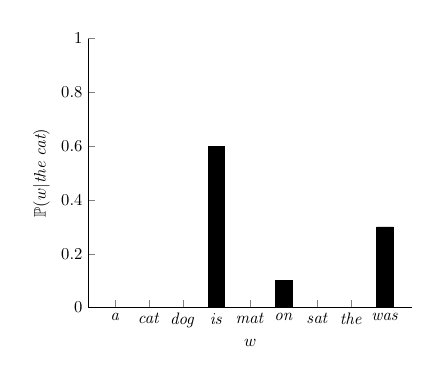
\begin{tikzpicture}[scale=0.6]
\begin{axis}[
	symbolic x coords={\tit{a}, \tit{cat}, \tit{dog}, \tit{is}, \tit{mat}, \tit{on}, \tit{sat}, \tit{the}, \tit{was}},
	xtick=data,
	xlabel={$w$},
	ylabel={$\mathbb{P}(w | \tit{the cat})$},
	ymin=0, ymax=1,
	axis x line*=bottom,
	axis y line*=left,
]

\addplot[ybar, fill=black]
coordinates {(\tit{a}, 0)(\tit{cat}, 0)(\tit{dog}, 0)(\tit{is}, 0.6)(\tit{mat}, 0)(\tit{on}, 0.1)(\tit{sat}, 0)(\tit{the}, 0)(\tit{was}, 0.3)};

\end{axis}
\end{tikzpicture}}}
~~\vcenter{\hbox{\scalebox{1}{$\rightarrow$}}}~~
\vcenter{\hbox{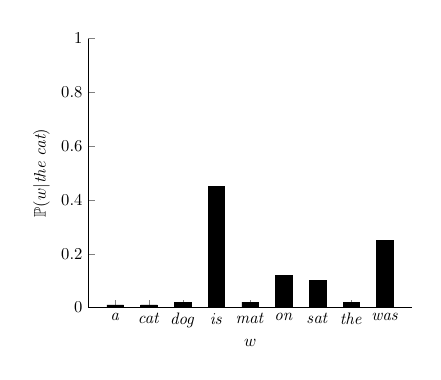
\begin{tikzpicture}[scale=0.6]
\begin{axis}[
	symbolic x coords={\tit{a}, \tit{cat}, \tit{dog}, \tit{is}, \tit{mat}, \tit{on}, \tit{sat}, \tit{the}, \tit{was}},
	xtick=data,
	xlabel={$w$},
	ylabel={$\mathbb{P}(w | \tit{the cat})$},
	ymin=0, ymax=1,
	axis x line*=bottom,
	axis y line*=left,
]

\addplot[ybar, fill=black]
coordinates {(\tit{a}, 0.01)(\tit{cat}, 0.01)(\tit{dog}, 0.02)(\tit{is}, 0.45)(\tit{mat}, 0.02)(\tit{on}, 0.12)(\tit{sat}, 0.1)(\tit{the}, 0.02)(\tit{was}, 0.25)};

\end{axis}
\end{tikzpicture}}}$
\caption{A toy example of smoothing. The probabilities of words that frequently follow \tit{`the cat'} are distributed to other less frequently occurring words in the vocabulary. The vocabulary is $V = \{$\tit{a}, \tit{cat}, \tit{dog}, \tit{is}, \tit{mat}, \tit{on}, \tit{sat}, \tit{the}, \tit{was}$\}$.}
\end{figure}

\subsection{Smoothing Techniques}

\subsubsection{Add-One Smoothing}

Add-one smoothing~\cite{add1_smoothing:johnson1932} simply involves adding 1 to each of the $n$-gram counts, and dividing by $|V|$ to ensure the probabilities sum to 1:
\begin{gather*}
	\mathbb{P}(w_i | w_{i - n + 1}^{i - 1})_{\text{\scshape add-one}} = \frac{c(w_{i - n + 1}^{i}) + 1}{\sum_w c(w_{i - n + 1}^{i - 1}w) + |V|}
\end{gather*}
One issue with add-one smoothing is that it gives an equal amount of probability to all $n$-grams, regardless of how likely they actually are. As an example, if both \tit{`the cat'} and \tit{`pizza cat'} are unseen in the training data of a bigram model, then $\mathbb{P}(\tit{cat}\ |\ \tit{the})_{\text{\scshape add-one}} = \mathbb{P}(\tit{cat}\ |\ \tit{pizza})_{\text{\scshape add-one}}$, despite the fact that \tit{`the'} is much more likely to precede \tit{`cat'} than \tit{`pizza'}. This problem can be reduced by employing \tit{backoff}, a technique whereby you recurse on the probability calculated by the $(n - 1)$-gram model. In this case, it is likely that $\mathbb{P}(\tit{the})_{\text{\scshape add-one}} > \mathbb{P}(\tit{pizza})_{\text{\scshape add-one}}$, which could be used to deduce that \tit{`the cat'} is more likely than \tit{`pizza cat'}.

\subsubsection{Absolute Discounting}

Absolute discounting employs backoff by interpolating higher and lower order $n$-gram models. It does this by subtracting a fixed discount $0 \leq D \leq 1$ from each non-zero count:
\begin{equation*}
\begin{aligned}
	\mathbb{P}(w_i | w_{i - n + 1}^{i - 1})_{\text{\scshape ABS}} &= \frac{max\{c(w_{i - n + 1}^{i}) - D, 0\}}{\sum_w c(w_{i - n + 1}^{i - 1}w)} \\
	&+ \frac{D}{\sum_w c(w_{i - n + 1}^{i - 1}w)}N_{1+}(w_{i - n + 1}^{i - 1}\bullet)\mathbb{P}(w_i | w_{i - n + 2}^{i - 1})_{\text{\scshape ABS}}
\end{aligned}
\end{equation*}
where
\begin{gather} \label{eq:n1plus}
	N_{1+}(w_{i - n + 1}^{i - 1}\bullet) = |\{ w\ |\ c(w_{i - n + 1}^{i - 1}w) \geq 1 \}|
\end{gather}
and the base case of recursion $\mathbb{P}(w)_{\text{\scshape ABS}}$ is given by the maximum likelihood unigram model. $N_{1+}(w_{i - n + 1}^{i - 1}\bullet)$ is the number of unique words that follow the sequence $w_{i - n + 1}^{i - 1}$, which is the number of $n$-grams that $D$ is subtracted from. It is not difficult to show that the coefficient attached to the $\mathbb{P}(w_i | w_{i - n + 2}^{i - 1})_{\text{\scshape ABS}}$ term ensures that the probabilities sum to 1. \\

Ney, Essen and Kneser~\cite{absolute_discounting:ney1994} suggested setting $D$ to the value:
\begin{gather} \label{eq:discount}
	D = \frac{n_1}{n_1 + 2n_2}
\end{gather}
where $n_1$ and $n_2$ are the total number of $n$-grams with 1 and 2 counts respectively.

\subsubsection{Kneser-Ney Smoothing}

Kneser and Ney proposed an extension to absolute discounting which takes into account the number of unique words that precede a given $n$-gram~\cite{kneser_ney_smoothing:kneser1995}. As a motivating example, consider the bigram \tit{`bottle cap'}. If \tit{`bottle cap'} has never been seen in the training data, then the absolute discounting model would backoff onto the unigram distribution for \tit{`cap'}. Using the unigram distribution, \tit{`Francisco'} might be given a higher probability than \tit{`cap'} (assuming \tit{`Francisco'} occurs more frequently than \tit{`cap'}). This would result in the bigram \tit{`bottle Francisco'} being given a higher probability than \tit{`bottle cap'}. Clearly, this is undesirable, because \tit{`Francisco'} only ever follows \tit{`San'}. \\

From this example, it seems intuitive to assign more probability to those $n$-grams that follow a larger number of unique words. Kneser and Ney encapsulate this intuition by replacing some of the absolute counts $c(w_i^j)$ with the number of unique words that precede the word sequence $w_i^j$, $N_{1+}(\bullet w_i^j)$:
\begin{gather*}
	N_{1+}(\bullet w_i^j) = |\{w\ |\ c(w_i^jw) \geq 1\}|
\end{gather*}
Kneser-Ney smoothing\footnote{This is actually the interpolated version of Kneser-Ney smoothing, which differs slightly in form to the equation presented in the original paper.} is defined as follows:
\begin{align*}
	\mathbb{P}(w_i | w_{i - n + 1}^{i - 1})_{\text{\scshape KN}} &= \frac{max\{\gamma(w_{i - n + 1}^{i}) - D, 0\}}{\sum_w \gamma(w_{i - n + 1}^{i - 1}w)} \\
	&+ \frac{D}{\sum_w \gamma(w_{i - n + 1}^{i - 1}w)}N_{1+}(w_{i - n + 1}^{i - 1}\bullet)\mathbb{P}(w_i | w_{i - n + 2}^{i - 1})_{\text{\scshape KN}}
\end{align*}
where
\begin{gather} \label{eq:gamma}
	\gamma(w_{i - k + 1}^i) = \begin{cases}
		c(w_{i - k + 1}^i) &\text{for the outermost level of recursion (i.e. $k = n$)} \\
		N_{1+}(\bullet w_{i - k + 1}^i) &\text{otherwise}
	\end{cases}
\end{gather}
and the unigram probability is given as:
\begin{gather*}
	\mathbb{P}(w_i)_{\text{\scshape KN}} = \frac{N_{1+}(\bullet w_i)}{\sum_w N_{1+}(\bullet w)}
\end{gather*}

\subsubsection{Modified Kneser-Ney Smoothing}

Chen and Goodman experimented with different discount values $D$ in Kneser-Ney smoothing and noticed that the ideal average discount value for $n$-grams with one or two counts is substantially different from the ideal average discount for $n$-grams with higher counts. Upon this discovery, they introduced a modified version of Kneser-Ney smoothing~\cite{modified_kneser_ney:chen1999}:
\begin{equation*}
\begin{aligned}
	\mathbb{P}(w_i | w_{i - k + 1}^{i - 1})_{\text{\scshape MKN}} &= \frac{max\{\gamma(w_{i - k + 1}^{i}) - D(c(w_{i - k + 1}^{i}), 0\}}{\sum_w \gamma(w_{i - k + 1}^{i - 1}w)} \\
	&+ \lambda(w_{i - k + 1}^{i - 1})\mathbb{P}(w_i | w_{i - k + 2}^{i - 1})_{\text{\scshape MKN}}
\end{aligned}
\end{equation*}
where $\gamma$ is defined in equation \ref{eq:gamma}, and $\lambda$ is defined as:
\begin{gather*}
	\lambda(w_{i - k + 1}^{i - 1}) = \frac{D_1N_1(w_{i - k + 1}^{i - 1}\bullet) + D_2N_2(w_{i - k + 1}^{i - 1}\bullet) + D_{3+}N_{3+}(w_{i - k + 1}^{i - 1}\bullet)}{\sum_w \gamma(w_{i - k + 1}^{i - 1}w)}
\end{gather*}
and
\begin{gather*}
	D(c) = \begin{cases}
		0 &\text{if }c = 0 \\
		D_1 &\text{if }c = 1 \\
		D_2 &\text{if }c = 2 \\
		D_{3+} &\text{if }c \geq 3 \\
	\end{cases}
\end{gather*}
where $N_1$, $N_2$ and $N_{3+}$ are defined analogously to $N_{1+}$ in equation~\ref{eq:n1plus}. Chen and Goodman suggest setting the discounts to be:
\begin{align*}
	D_1 = 1 - 2D\frac{n_2}{n_1} && D_2 = 2 - 3D\frac{n_3}{n_2} && D_{3+} = 3 - 4D\frac{n_4}{n_3}
\end{align*}
where $D$ is as defined in equation \ref{eq:discount}.

\subsubsection{Katz Smoothing}

Katz smoothing is a popular smoothing technique based on the Good-Turing estimate~\cite{good_turing:good1953}. The Good-Turing estimate states an $n$-gram that occurs $r$ times should be treated as occurring $r^*$ times, where:
\begin{gather*}
	r^* = (r + 1)\frac{n_{r + 1}}{n_r}
\end{gather*}
where $n_r$ is the number of $n$-grams that occur $r$ times. Converting this count into a probability simply involves normalising as follows:
\begin{gather} \label{eq:gt}
	\mathbb{P}(w_i | w_{i - n + 1}^{i - 1})_{\text{\scshape GT}} = \frac{c^*(w_{i - n + 1}^{i})}{\sum_{r = 0}^\infty n_r r^*}
\end{gather}
Katz smoothing~\cite{katz_smoothing:katz1987} is then defined as:
\begin{gather} \label{eq:katz}
	\mathbb{P}(w_i | w_{i - n + 1}^{i - 1})_{\text{\scshape KATZ}} = \begin{cases}
		\mathbb{P}(w_i | w_{i - n + 1}^{i - 1})_{\text{\scshape GT}} &\text{if }c(w_{i - n + 1}^i) > 0 \\
		\alpha(w_{i - n + 1}^{i - 1})\mathbb{P}(w_i | w_{i - n + 2}^{i - 1})_{\text{\scshape KATZ}} &\text{otherwise}
	\end{cases}
\end{gather}
where
\begin{gather*}
	\alpha(w_{i - n + 1}^{i - 1}) = \frac{1 - \sum_{\{w_i\ |\ c(w_{i - n + 1}^i) > 0\}} \mathbb{P}(w_i | w_{i - n + 1}^{i - 1})_{\text{\scshape KATZ}}}{1 - \sum_{\{w_i\ |\ c(w_{i - n + 1}^i) > 0\}} \mathbb{P}(w_i | w_{i - n + 2}^{i - 1})_{\text{\scshape KATZ}}}
\end{gather*}
In practice, the infinite sum in equation \ref{eq:gt} cannot be computed. To get around this issue, Katz takes $n$-gram counts above some threshold $k$ as reliable and only applies the Good-Turing estimate to those with a count less than or equal to $k$. Katz suggests $k = 5$. This modification requires a slightly different equation to \ref{eq:katz} and is presented in Katz's original paper.

\section{Recurrent Neural Network Models}

In this section I give a brief introduction to neural networks, recurrent neural networks (RNNs) and how RNNs can be used in the context of language modelling. A thorough description of the more complex RNN architectures, gated recurrent units (GRUs) and long short-term memory (LSTM), is given in chapter \ref{implementation}.

\subsection{An Overview of Neural Networks}

The human brain is a furiously complicated organ, packed with a network of approximately 86 billion neurons\footnote{According to a study by Azevedo et al.~\cite{brain_size:azevedo2009}.} that propagate electrochemical signals across connections called synapses. Artificial neural networks, or neural networks, were originally developed as a mathematical model of the brain~\cite{nn_calculus:mcculloch1943}, which despite being substantially oversimplified, now provides an effective tool for classification and regression in modern-day machine learning. \\

\tikzset{
	every neuron/.style={
		circle,
		draw,
		minimum size=5mm
	},
	neuron missing/.style={
		draw=none,
		scale=2,
		text height=0.1cm,
		execute at begin node=\color{black}$\hdots$
	},
}

%\begin{figure}[h]
%\begin{center}
%\begin{tikzpicture}[x=1.5cm, y=1.5cm, >=stealth]

%\foreach \m/\l [count=\y] in {1, 2, 3, missing, 4}
%	\node [every neuron/.try, neuron \m/.try] (input-\m) at (0, 2.5-\y) {};

%\foreach \m [count=\y] in {1, missing, 2}
%	\node [every neuron/.try, neuron \m/.try ] (hidden-\m) at (1.5, 2-\y*1.25) {};

%\foreach \m [count=\y] in {1, missing, 2}
%	\node [every neuron/.try, neuron \m/.try ] (hidden-2-\m) at (3, 2-\y*1.25) {};

%\foreach \m [count=\y] in {1, missing, 2}
%	\node [every neuron/.try, neuron \m/.try ] (output-\m) at (4.5, 1.5-\y) {};

%\foreach \l [count=\i] in {1, 2, 3, n}
%	\draw [<-] (input-\i) -- ++(-1,0) node [above, midway] {$x_\l$};

%\foreach \l [count=\i] in {1, m}
%	\draw [->] (output-\i) -- ++(1,0) node [above, midway] {$y_\l$};

%\foreach \i in {1, ..., 4}
%	\foreach \j in {1, ..., 2}
%		\draw [->] (input-\i) -- (hidden-\j);

%\foreach \i in {1, ..., 2}
%	\foreach \j in {1, ..., 2}
%		\draw [->] (hidden-\i) -- (hidden-2-\j);

%\foreach \i in {1, ..., 2}
%	\foreach \j in {1, ..., 2}
%		\draw [->] (hidden-2-\i) -- (output-\j);

%\foreach \l [count=\x from 0] in {Input, Hidden, Hidden, Output}
%	\node [align=center, above] at (\x*1.5, 2) {\l \\ layer};

%\end{tikzpicture}
%\caption{An example multilayer perceptron, with two hidden layers.}
%\end{center}
%\end{figure}

\begin{figure}[h]
\captionsetup{justification=centering}
\centering
\begin{subfigure}{0.5\linewidth}
	\centering
	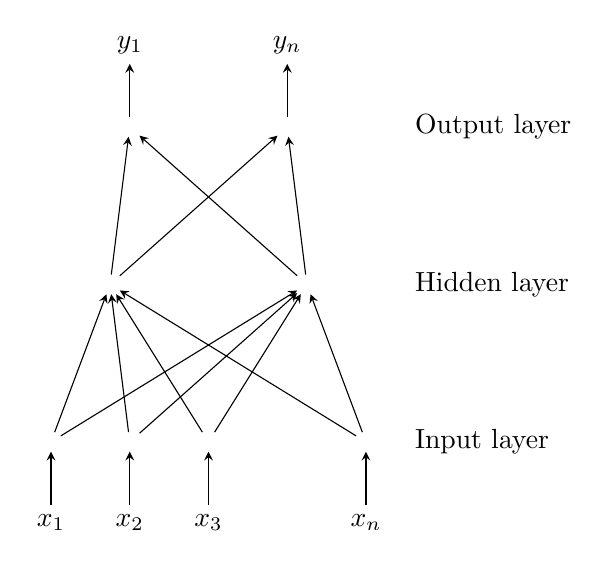
\begin{tikzpicture}[>=stealth]

	\foreach \m/\l [count=\x] in {1, 2, 3, missing, 4}
		\node [every neuron/.try, neuron \m/.try] (input-\m) at (\x - 2.5, 0) {};

	\foreach \m [count=\x] in {1, missing, 2}
		\node [every neuron/.try, neuron \m/.try ] (hidden-\m) at (\x*1.25 - 2, 2) {};

	\foreach \m [count=\x] in {1, missing, 2}
		\node [every neuron/.try, neuron \m/.try ] (output-\m) at (\x - 1.5, 4) {};

	\foreach \l [count=\i] in {1, 2, 3, n}
		\draw [<-] (input-\i) -- ++(0, -0.8) node [below] {$x_\l$};

	\foreach \l [count=\i] in {1, n}
		\node [above] at (hidden-\i.north) {};

	\foreach \l [count=\i] in {1, n}
		\draw [->] (output-\i) -- ++(0, 0.8) node [above] {$y_\l$};

	\foreach \i in {1, ..., 4}
		\foreach \j in {1, ..., 2}
			\draw [->] (input-\i) -- (hidden-\j);

	\foreach \i in {1, ..., 2}
		\foreach \j in {1, ..., 2}
			\draw [->] (hidden-\i) -- (output-\j);

	\foreach \l [count=\y from 0] in {Input, Hidden, Output}
		\node [right] at (3, \y*2) {\l\ layer};
	\end{tikzpicture}
	\caption{An example multilayer perceptron.}
\end{subfigure}%
\begin{subfigure}{0.5\linewidth}
	\centering
	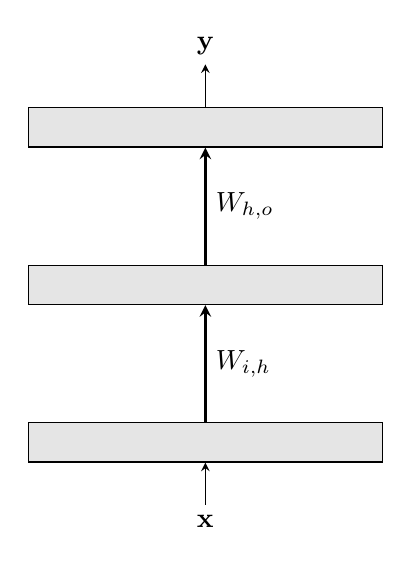
\begin{tikzpicture}[>=stealth]
		\node[draw, rectangle, minimum width=45mm, minimum height=5mm, fill=black!10, ] (input) at (0, 0) {};
		\node[draw, rectangle, minimum width=45mm, minimum height=5mm, fill=black!10] (hidden) at (0, 2) {};
		\node[draw, rectangle, minimum width=45mm, minimum height=5mm, fill=black!10] (output) at (0, 4) {};
		\draw [<-] (input) -- ++(0, -0.8) node [below] {$\mathbf{x}$};
		\draw [->, line width=0.3mm] (input) to node [right] {$W_{i,h}$} (hidden);
		\draw [->, line width=0.3mm] (hidden) to node [right] {$W_{h,o}$} (output);
		\draw [->] (output) -- ++(0, 0.8) node [above] {$\mathbf{y}$};
	\end{tikzpicture}
	\caption{A simplified notation for (a).}
\end{subfigure}
\caption{Two alternative notations for the same network: a multilayer perceptron with one hidden layer. In the simplified notation, the grey rectangle represents a vector of neurons, the thin arrow represents a vector and the thick arrow represents a matrix of weights.}
\end{figure}

Neural networks consist of a series of nodes which are joined by directed and weighted connections. Inputs are supplied to some subset of the nodes and then propagated along the weighted connections until they reach the designated output nodes. In the context of the brain, the nodes represent neurons, the weighted connections represent synapses and the flow of information represents electrochemical signals. \\

An important distinction to be made is whether the neural network is cyclic or not. Acyclic neural networks are called feed-forward neural networks (FNNs), whereas cyclic neural networks are denoted recurrent neural networks (RNNs) which are covered in section \ref{rnns}. There are a variety of FNNs, but the most prominent is the multilayer perceptron (MLP)~\cite{backprop:rumelhart1985}, which I will outline below. \\

\subsubsection{The Multilayer Perceptron}

The multilayer perceptron consists of layers of neurons, where each layer is fully connected to the next one. The first layer is the input layer, the last is the output layer and any layers in between are called \tit{hidden layers}. If there is more than one hidden layer then it is called a \tit{deep} neural network. The input neurons simply pass on the input values that they are given. The neurons in the subsequent layers of the network compute the weighted sum of their inputs, before passing that value through an \tit{activation function} and outputting it:

\begin{figure}[h]
\captionsetup{justification=centering}
\begin{center}
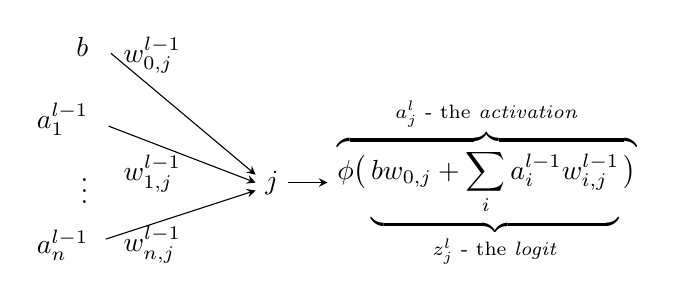
\begin{tikzpicture}[x=1.5cm, y=1.5cm, >=stealth]

\node[every neuron/.try] (neuron) {$j$};
\node[left=10mm of neuron] (mid) {};
\node[above left=12mm and 20mm of neuron] (bias) {$b$};
\node[above left=2mm and 20mm of neuron] (inp1) {$a_1^{l-1}$};
\node[left=20mm of neuron] (var) {$\vdots$};
\node[below left=2mm and 20mm of neuron] (inpN) {$a_n^{l-1}$};

\draw[<-] (neuron.west |- mid) coordinate (aux)--++(159:20mm) node [below right=0mm and 2mm of inp1] {$w_{1,j}^{l-1}$};
\draw[<-] ([yshift=1mm]aux)--++(140:24mm) node [below right=-5mm and 2mm of bias] {$w_{0,j}^{l-1}$};
\draw[<-] ([yshift=-1mm]aux)--++(-162:20mm) node [right=2mm of inpN] {$w_{n,j}^{l-1}$};

\draw[->] (neuron.east) -- ++(0:5mm) node [right] {$\overbrace{\phi \big( \underbrace{bw_{0,j} + \sum_i a_i^{l - 1} w_{i,j}^{l-1}}_{z_j^l\text{ - the \tit{logit}}} \big)}^{a_j^l\text{ - the \tit{activation}}}$};

\end{tikzpicture}
\caption{The computation carried out by each neuron. The outputs or \tit{activations} of the neurons from the previous layer, $(l - 1)$, are denoted $a_i^{l-1}$, the weights on the input connections are $w_{i,j}^{l-1}$, the activation function is $\phi$ and $b$ is the bias input.}
\label{fig:neuron}
\end{center}
\end{figure}

The unusual looking input $b$ is a \tit{bias} input. This is a fixed-value input, typically set to 1, which allows the neuron to shift the output of the activation function left and right by adjusting the weight $w_0$. Bias inputs are usually attached to every non-input neuron in the network. \\

It is also worth noting that activation functions should be chosen to be non-linear. Any combination of linear operators is linear, which means that any linear MLP with multiple hidden layers is equivalent to an MLP with a single hidden layer. Non-linear neural networks, on the other hand, are more powerful, and can gain considerable performance by adding successive hidden layers to re-represent the input data at higher levels of abstraction~\cite{dbn:hinton2006}~\cite{scaling:bengio2007}. In fact, is has been shown that a non-linear MLP with a single hidden layer containing a sufficient number of neurons can approximate any continuous function on a compact input domain to arbitrary precision~\cite{universal_approximators:hornik1989}. \\

Frequently used activation functions include the sigmoid and the hyperbolic tangent functions. These are both non-linear functions squashed within the ranges $(0, 1)$ and $(-1, 1)$ respectively. Their steep slope at the origin is supposed to mimic an axon, which fires its output after the input reaches a certain potential. More importantly, these functions are differentiable, which allows for the network to be trained using gradient descent. This is discussed below. \\

\begin{figure}[h]
\captionsetup{justification=centering}
\centering
\begin{subfigure}{0.5\linewidth}
	\centering
	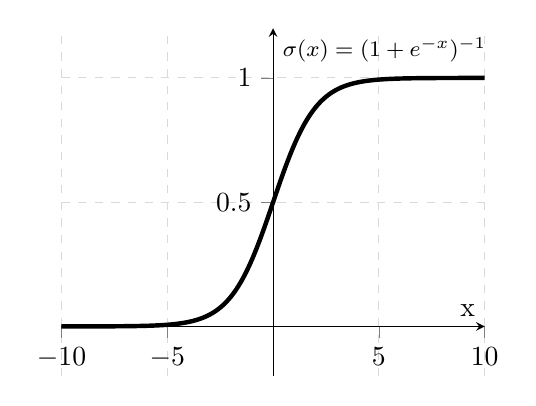
\begin{tikzpicture}
	\begin{axis}[
		height=6cm,
		legend pos=north west,
		axis x line=middle,
		axis y line=middle,
		grid = major,
		grid style={dashed, gray!30},
		xmin=-10, xmax= 10,
		ymin= -0.2, ymax= 1.2,
		xlabel=x,
		ylabel={\footnotesize $\sigma(x) = (1 + e^{-x})^{-1}$},
		tick align=outside,
		enlargelimits=false]
	\addplot[domain=-10:10, black, ultra thick,samples=500] {1/(1+exp(-x))};
	\end{axis}
	\end{tikzpicture}
	\caption{The sigmoid function, $\sigma$.}
\end{subfigure}%
\begin{subfigure}{0.5\linewidth}
	\centering
	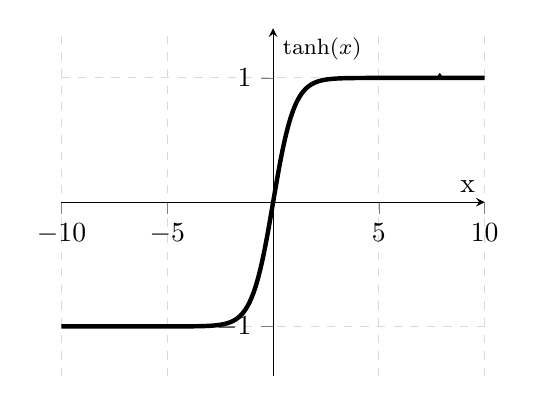
\begin{tikzpicture}
	\begin{axis}[
		height=6cm,
		legend pos=north west,
		axis x line=middle,
		axis y line=middle,
		grid = major,
		grid style={dashed, gray!30},
		xmin=-10, xmax= 10,
		ymin= -1.4, ymax= 1.4,
		xlabel=x,
		ylabel={\footnotesize $\tanh (x)$},
		tick align=outside,
		enlargelimits=false]
	\addplot[domain=-10:10, black, ultra thick,samples=500] {(exp(x) - exp(-x))/(exp(x) + exp(-x))};
	\end{axis}
	\end{tikzpicture}
	\caption{The hyperbolic tangent function, $\tanh$.}
\end{subfigure}
\caption{Two popular activation functions.}
\end{figure}

\subsubsection{Backpropagation and Gradient Descent}

FNNs compute a function, $f$, parameterised by the weights $\mathbf{w}$ of the network, mapping an input vector $\mathbf{x} = (x_1, ..., x_n)^T$ to an output vector $\mathbf{y} = (y_1, ..., y_m)^T$. 
\begin{gather*}
	\mathbf{y} = f_\mathbf{w}(\mathbf{x})
\end{gather*}
The entire point of training a neural network is to get it to learn a particular mapping from input vectors to output vectors. What the inputs and outputs represent depends on the problem at hand. For example, in the context of classifying pictures of animals, the input vector might represent the pixel values of an image and the output vector might represent a probability distribution over the set of animals in the classification task. \\

In order to train a neural network, you supply it with a training set, which is just a list of input-target pairs:
\begin{gather*}
	\mathbf{s} = ((\mathbf{x}_1, \mathbf{t}_1), ..., (\mathbf{x}_N, \mathbf{t}_N))
\end{gather*}
Where $\mathbf{t}_i$ is the vector that the network should output given the example input $\mathbf{x}_k$. A differentiable loss function, $\mathcal{L}(\mathbf{y}, \mathbf{t})$, is also defined, which essentially says how badly the network output $\mathbf{y}$ matches the target output $\mathbf{t}$. Then, a measure of how much error the network produces over the whole training set can be defined as follows:
\begin{gather*}
	\mathcal{L}_{\text{\scshape total}} = \sum_{k = 1}^N \mathcal{L}(f_{\mathbf{w}}(\mathbf{x}_k), \mathbf{t}_k)
\end{gather*}
The end product of the \tit{backpropagation} algorithm is the partial derivative:
\begin{gather*}
	\frac{\partial}{\partial w_{i,j}^l} \big( \mathcal{L}_{\text{\scshape total}} \big)
\end{gather*}
for every weight $w_{i,j}^l$ in the neural network. It is a two stage algorithm that works as follows:
\begin{enumerate}
\item
	Calculate, $f_{\mathbf{w}}(\mathbf{x}_k)$ for each input example $\mathbf{x}_k$, and use those values to derive $\mathcal{L}_{\text{\scshape total}}$. The process of calculating the output of the neural network given the input is known as \tit{forward propagation}, because the input is propagated through each layer in the network.
\item
	Given $\mathcal{L}_{\text{\scshape total}}$, calculate $\frac{\partial}{\partial w_{i,j}^l} \big( \mathcal{L}_{\text{\scshape total}} \big)$ for each weight in each layer of the network by applying the chain rule backwards from the output layer to the input layer. This step is described in more detail below.
\end{enumerate}

$\frac{\partial}{\partial w_{i,j}^l} \big( \mathcal{L}_{\text{\scshape total}} \big)$ is calculated as follows:
\begin{gather} \label{eq:bp_weight_grad}
	\frac{\partial}{\partial w_{i,j}^l} \big( \mathcal{L}_{\text{\scshape total}} \big) = \sum_{k = 1}^N \underbrace{\frac{\partial \mathcal{L}}{\partial f_{\mathbf{w}}(\mathbf{x}_k)}  \frac{\partial f_{\mathbf{w}}(\mathbf{x}_k)}{\partial z_j^{l + 1}}}_{\delta_j^{l+1}}  \frac{\partial z_j^{l + 1}}{\partial w_{i,j}^l} = \delta_j^{l+1} a_i^l
\end{gather}
The term $\delta_j^{l+1}$ varies in form for each layer. For the output layer, it has the following form:
\begin{gather} \label{eq:delta_output}
	\delta_j^L = \frac{\partial \mathcal{L}}{\partial f_{\mathbf{w}}(\mathbf{x}_k)} \phi'(z_j^L)
\end{gather}
For the preceding layers, $\delta_j^l$ can be defined recursively in terms of the delta values for the neurons in subsequent layers in the network. This is defined below, and a detailed justification of it is given in appendix \ref{appendix:bp_recurrence}:
\begin{gather} \label{eq:delta_hidden}
	\delta_i^l = \phi'(z_i^l) \sum_j \delta_j^{l+1} w_{i,j}^l
\end{gather}

\tit{Gradient descent} is an optimisation technique that uses the derivatives produced by the backpropagation algorithm to adjust the weights such that the loss is minimised over the training set. The simplest form of gradient descent does this by changing each weight value in the direction of the negative gradient of the loss. This is is equivalent to moving the network output downwards on the error surface defined by plotting the loss against each of the weights in the network:
\begin{gather*}
	w_{i,j}^l \leftarrow w_{i,j}^l - \eta \frac{\partial}{\partial w_{i,j}^l} \big( \mathcal{L}_{\text{\scshape total}} \big)
\end{gather*}
$\eta$ is known as the \tit{learning rate}, which determines how large the steps are in the negative direction of the gradient. Ways for setting $\eta$, and other useful techniques when training neural networks in practice are described in chapter \ref{implementation}.

\subsection{Recurrent Neural Networks} \label{rnns}

In the context of language modelling, the input is a sequence of words and the output should be the same sequence of words shifted ahead in time by one word. For example, given (\tit{`the', `cat', `sat', ...}) as input, the network should produce something similar to (\tit{`cat', `sat', `on', ...}) as output. The problem with FNNs is that these sequences may have a varying number of words in them, yet FNNs have fixed input and output vector sizes. One way to get around this problem is to look at a finite window of words at any given time, and encode that window into a vector, but even for modest window sizes this can lead to a huge number of weights in the network, which becomes more difficult to train. A better solution is to use a recurrent neural network.

\begin{figure}[h]
\captionsetup{justification=centering}
\centering
\begin{subfigure}{0.3\linewidth}
	\centering
	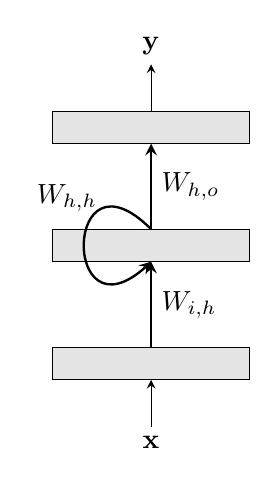
\begin{tikzpicture}[>=stealth]
		\node[draw, rectangle, minimum width=25mm, minimum height=4mm, fill=black!10, ] (input) at (0, 0) {};
		\node[draw, rectangle, minimum width=25mm, minimum height=4mm, fill=black!10] (hidden) at (0, 1.5) {};
		\node[draw, rectangle, minimum width=25mm, minimum height=4mm, fill=black!10] (output) at (0, 3) {};
		\draw [<-] (input) -- ++(0, -0.8) node [below] {$\mathbf{x}$};
		\draw [->, line width=0.3mm] (input) to node [right] {$W_{i,h}$} (hidden);
		\draw [->, line width=0.3mm, out=135, in=225, looseness=10] (hidden.north) to node [above left=3mm and -3mm of hidden] {$W_{h,h}$} (hidden.south);
		\draw [->, line width=0.3mm] (hidden) to node [right] {$W_{h,o}$} (output);
		\draw [->] (output) -- ++(0, 0.8) node [above] {$\mathbf{y}$};
	\end{tikzpicture}
	\caption{An RNN.}
	\label{fig:rnn}
\end{subfigure}%
\begin{subfigure}{0.7\linewidth}
	\centering
	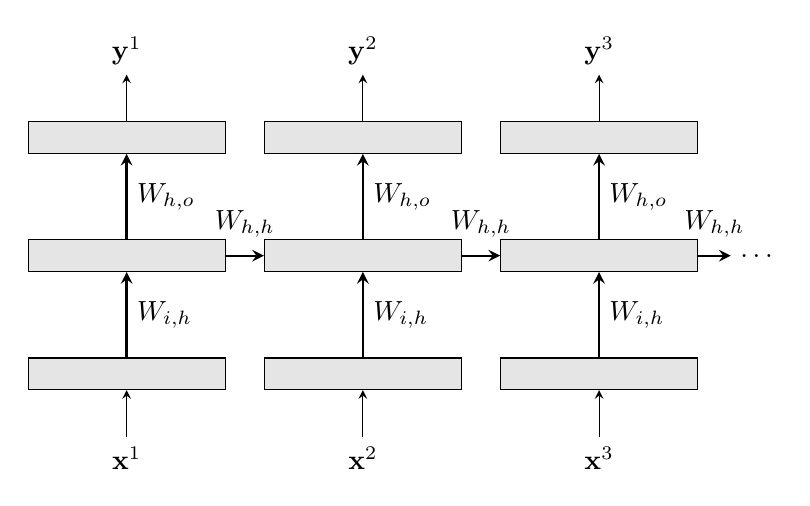
\begin{tikzpicture}[>=stealth]
		\node[draw, rectangle, minimum width=25mm, minimum height=4mm, fill=black!10, ] (input1) at (0, 0) {};
		\node[draw, rectangle, minimum width=25mm, minimum height=4mm, fill=black!10] (hidden1) at (0, 1.5) {};
		\node[draw, rectangle, minimum width=25mm, minimum height=4mm, fill=black!10] (output1) at (0, 3) {};
		\draw [<-] (input1) -- ++(0, -0.8) node [below] {$\mathbf{x}^1$};
		\draw [->, line width=0.3mm] (input1) to node [right] {$W_{i,h}$} (hidden1);
		\draw [->, line width=0.3mm] (hidden1) to node [right] {$W_{h,o}$} (output1);
		\draw [->] (output1) -- ++(0, 0.8) node [above] {$\mathbf{y}^1$};

		\node[draw, rectangle, minimum width=25mm, minimum height=4mm, fill=black!10, ] (input2) at (3, 0) {};
		\node[draw, rectangle, minimum width=25mm, minimum height=4mm, fill=black!10] (hidden2) at (3, 1.5) {};
		\node[draw, rectangle, minimum width=25mm, minimum height=4mm, fill=black!10] (output2) at (3, 3) {};
		\draw [<-] (input2) -- ++(0, -0.8) node [below] {$\mathbf{x}^2$};
		\draw [->, line width=0.3mm] (input2) to node [right] {$W_{i,h}$} (hidden2);
		\draw [->, line width=0.3mm] (hidden2) to node [right] {$W_{h,o}$} (output2);
		\draw [->] (output2) -- ++(0, 0.8) node [above] {$\mathbf{y}^2$};

		\node[draw, rectangle, minimum width=25mm, minimum height=4mm, fill=black!10, ] (input3) at (6, 0) {};
		\node[draw, rectangle, minimum width=25mm, minimum height=4mm, fill=black!10] (hidden3) at (6, 1.5) {};
		\node[draw, rectangle, minimum width=25mm, minimum height=4mm, fill=black!10] (output3) at (6, 3) {};
		\draw [<-] (input3) -- ++(0, -0.8) node [below] {$\mathbf{x}^3$};
		\draw [->, line width=0.3mm] (input3) to node [right] {$W_{i,h}$} (hidden3);
		\draw [->, line width=0.3mm] (hidden3) to node [right] {$W_{h,o}$} (output3);
		\draw [->] (output3) -- ++(0, 0.8) node [above] {$\mathbf{y}^3$};

		\node (cont) at (8, 1.5) {$\hdots$};

		\draw [->, line width=0.3mm] (hidden1.east) to node [above=1mm of hidden1] {$W_{h,h}$} (hidden2.west);
		\draw [->, line width=0.3mm] (hidden2.east) to node [above=1mm of hidden2] {$W_{h,h}$} (hidden3.west);
		\draw [->, line width=0.3mm] (hidden3.east) to node [above=1mm of hidden3] {$W_{h,h}$} (cont.west);
	\end{tikzpicture}
	\caption{An unrolled RNN.}
	\label{fig:rnn_unrolled}
\end{subfigure}
\caption{Two different representations of the same RNN.}
\end{figure}

A recurrent neural network can be constructed from an FNN by adding connections from each neuron in a hidden layer back to every neuron in that layer, including itself. This gives something like the network shown in figure \ref{fig:rnn}. An easier way to visualise an RNN is by \tit{unrolling} it as shown in figure \ref{fig:rnn_unrolled}. A nice property about RNNs is that they can be unrolled an arbitrary number of steps without the need for any additional parameters, because the same weight matrices are reused at each step. For this reason, RNNs are well suited for operating over sequences of input data. In the case of language modelling, this is ideal, because the inputs are sequences of words. The problem of representing textual words as numerical input vectors for an RNN is addressed in section \ref{word_embeddings}. \\

As shown in figure \ref{fig:rnn_unrolled}, RNNs can take a sequence of vectors as input. In most applications, the vectors in such sequences are typically ordered by time, so I use the notation $\mathbf{x}^t$ and $\mathbf{y}^t$ to denote the input and output vectors at time step $t$.

\subsubsection{Backpropagation Through Time (BPTT)}

Training an RNN is not so much different to training an FNN: the only difference is that gradients must also be calculated across time steps. As shown figure \ref{fig:rnn_unrolled}, each weight is reused at each time step. For this reason, the weight update given in equation \ref{eq:bp_weight_grad} is summed across the time steps:
\begin{gather*}
	\frac{\partial}{\partial w_{i,j}^l} \big( \mathcal{L}_{\text{\scshape total}} \big) = \sum_t \delta_j^{l+1,t} a_i^{l,t}
\end{gather*}
The delta term for the output layer is defined analogously to equation \ref{eq:delta_output}:
\begin{gather} \label{eq:delta_output}
	\delta_j^{L,t} = \frac{\partial \mathcal{L}}{\partial f_{\mathbf{w}}(\mathbf{x}_k^t)} \phi'(z_j^{L,t})
\end{gather}
The delta term for the preceding layers can be shown to have the form below. This is justified in more detail in appendix \ref{appendix:bp_recurrence}.
\begin{gather} \label{eq:delta_hidden}
	\delta_i^{l,t} = \phi'(z_i^{l,t}) \big( \sum_j \delta_j^{l+1,t} w_{i,j}^l + \sum_j \delta_j^{l,t+1} v_{i,j}^l \big)
\end{gather}
where $v_{i,j}^l$ denotes the weight on the recurrent connection from neuron $i$ in layer $l$ back to neuron $j$ in the same layer.

\subsubsection{Vanilla Recurrent Neural Networks}
So far, the equations presented have assumed a \tit{vanilla RNN}. That is, each neuron, or \tit{cell}, simply computes the weighted sum of its inputs and then applys an activation function. A significant problem associated with this architecture is known as the \tit{vanishing gradient problem}. Namely, the influence of a particular input on the hidden layers and subsequently the output layer either decays or blows up exponentially as it cycles through the recurrent connections, which makes it difficult for this architecture to retain long-term information across several steps. Various improvements have been made to improve upon this problem, two of which are outlined below.

\subsubsection{Long Short-Term Memory}
The most effective solution so far for tackling the vanishing gradient problem is the Long Short-Term Memory architecture proposed by Hochreiter and Schmidhuber~\cite{lstm:hochreiter1997}. In their architecture, each cell maintains a state, $\mathbf{c}$, which is manipulated according to the inputs it receives to produce a new state and the cell output. At each cell, the state passes through three gates: the \tit{forget gate}, \tit{input gate} and the \tit{output gate}. The effect of such gates and a more detailed discussion of this architecture is given in chapter~\ref{implementation}.

\begin{figure}[h]
\centering
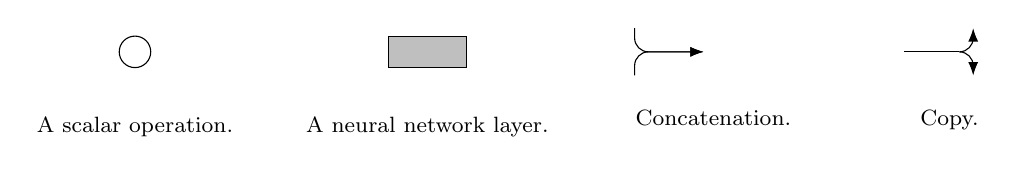
\begin{tikzpicture}[
	scalar/.style={circle, draw, inner sep=0pt, minimum width=4mm},
	tanlayer/.style={rectangle, draw, inner sep=0pt, fill=gray!50, minimum width=10mm, minimum height=4mm},
	siglayer/.style={rectangle, draw, inner sep=0pt, fill=gray!50, minimum width=6mm, minimum height=4mm},
	textb/.style={minimum width=6mm, minimum height=4mm},
	ct/.style={circle, draw, inner sep=5pt, ultra thick, minimum width=10mm},
	ft/.style={circle, draw, minimum width=8mm, inner sep=1pt},
	filter/.style={circle, draw, minimum width=7mm, inner sep=1pt, path picture={\draw[thick, rounded corners] (path picture bounding box.center)--++(65:2mm)--++(0:1mm);
	\draw[thick, rounded corners] (path picture bounding box.center)--++(245:2mm)--++(180:1mm);}},
	mylabel/.style={font=\scriptsize\sffamily},
	>=LaTeX
]

\node[tanlayer] (nnlayer) {};
\node[textb, below=5mm of nnlayer] (nnlayertext) {\footnotesize A neural network layer.};
\node[scalar, left=30mm of nnlayer] (scalar) {};
\node[textb, below=5mm of scalar] (scalartext) {\footnotesize A scalar operation.};
\node[right=30mm of nnlayer] (concat) {};
\node[textb, below=5mm of concat] (concattext) {\footnotesize Concatenation.};
\node[right=60mm of nnlayer] (copy) {};
\node[textb, below=5mm of copy] (copytext) {\footnotesize Copy.};

\draw[<-, rounded corners=5pt] (concat) -| ++(-10mm,3mm);
\draw[<-, rounded corners=5pt] (concat) -| ++(-10mm,-3mm);

\draw[rounded corners=5pt] (copy.east) -- ++(-7mm,0mm);
\draw[->, rounded corners=5pt] (copy) -| ++(3mm,3mm);
\draw[->, rounded corners=5pt] (copy) -| ++(3mm,-3mm);

\end{tikzpicture}
\caption{A notation for drawing RNN architectures.}
\label{fig:rnn_notation}
\end{figure}

\subsubsection{Gated Recurrent Unit}
Whilst the LSTM architecture provides a significant improvement for retaining long-term information, it is computationally more expensive to run. Cho et al.\ propose the Gated Recurrent Unit~\cite{gru:cho2014}, which is a simplified version of LSTM that is cheaper to compute. The most significant changes are that it combines the forget and input gates into a single `update gate', and it merges the cell state and cell output. This architecture is also described in more detail in chapter~\ref{implementation}.

\begin{figure}[h]
\centering
\begin{subfigure}{0.33\linewidth}
	\centering
	\resizebox{4cm}{3cm}{%
	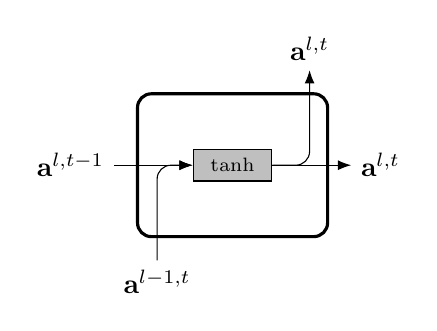
\begin{tikzpicture}[
		scalar/.style={circle, draw, inner sep=0pt, minimum width=4mm},
		tanlayer/.style={rectangle, draw, inner sep=0pt, fill=gray!50, minimum width=10mm, minimum height=4mm},
		siglayer/.style={rectangle, draw, inner sep=0pt, fill=gray!50, minimum width=6mm, minimum height=4mm},
		textb/.style={minimum width=6mm, minimum height=4mm},
		ct/.style={circle, draw, inner sep=5pt, ultra thick, minimum width=10mm},
		ft/.style={circle, draw, minimum width=8mm, inner sep=1pt},
		filter/.style={circle, draw, minimum width=7mm, inner sep=1pt, path picture={\draw[thick, rounded corners] (path picture bounding box.center)--++(65:2mm)--++(0:1mm);
		\draw[thick, rounded corners] (path picture bounding box.center)--++(245:2mm)--++(180:1mm);}},
		mylabel/.style={font=\scriptsize\sffamily},
		>=LaTeX
	]
	
	\node[tanlayer] (tanh) {\scriptsize $\tanh$};
	\node[textb, anchor=east, left=10mm of tanh] (hin) {$\mathbf{a}^{l, t - 1}$};
	\node[textb, anchor=west, right=10mm of tanh] (hout) {$\mathbf{a}^{l, t}$};
	\node[textb, anchor=north, below left=10mm and -1mm of tanh] (x) {$\mathbf{a}^{l - 1, t}$};
	\node[textb, anchor=south, above right=10mm and 1mm of tanh] (hout2) {$\mathbf{a}^{l, t}$};
	\node[fit=(tanh), draw, inner xsep=7mm, inner ysep=7mm, rounded corners=5pt, line width=0.4mm] (fit) {};

	\foreach \i/\j in {hin/tanh.west, tanh.east/hout}
		\draw[->, rounded corners=5pt] (\i) -- (\j);

	\draw [->, rounded corners=5pt] (x.north) |- (tanh.west);

	\draw [->, rounded corners=5pt] (tanh.east) -| (hout2);

	\end{tikzpicture}}
	\caption{A vanilla RNN cell.}
\end{subfigure}%
\begin{subfigure}{0.33\linewidth}
	\centering
	\resizebox{4.8cm}{3cm}{%
	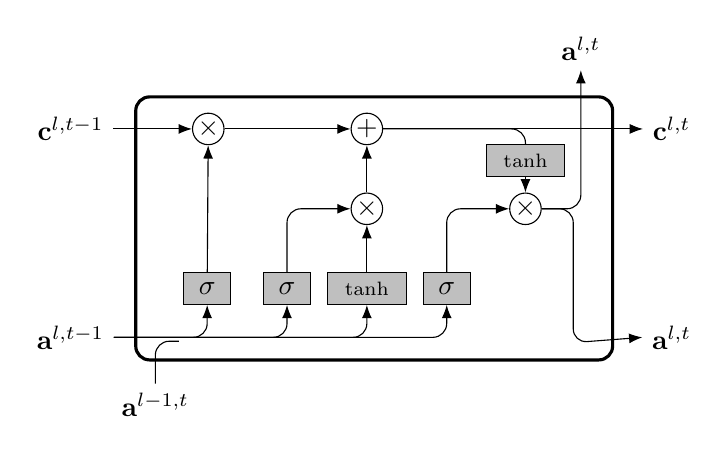
\begin{tikzpicture}[
		scalar/.style={circle, draw, inner sep=0pt, minimum width=4mm},
		tanlayer/.style={rectangle, draw, inner sep=0pt, fill=gray!50, minimum width=10mm, minimum height=4mm},
		siglayer/.style={rectangle, draw, inner sep=0pt, fill=gray!50, minimum width=6mm, minimum height=4mm},
		textb/.style={minimum width=6mm, minimum height=4mm},
		ct/.style={circle, draw, inner sep=5pt, ultra thick, minimum width=10mm},
		ft/.style={circle, draw, minimum width=8mm, inner sep=1pt},
		filter/.style={circle, draw, minimum width=7mm, inner sep=1pt, path picture={\draw[thick, rounded corners] (path picture bounding box.center)--++(65:2mm)--++(0:1mm);
		\draw[thick, rounded corners] (path picture bounding box.center)--++(245:2mm)--++(180:1mm);}},
		mylabel/.style={font=\scriptsize\sffamily},
		>=LaTeX
	]
	
	\node[scalar] (plus) {$+$};
	\node[scalar, left=16mm of plus] (ftimes) {$\times$};
	\node[scalar, below=6mm of plus] (itimes) {$\times$};
	\node[scalar, right=16mm of itimes] (otimes) {$\times$};
	\node[tanlayer, above=2mm of otimes] (otanh) {\scriptsize $\tanh$};
	\node[tanlayer, below=6mm of itimes] (stanh) {\scriptsize $\tanh$};
	\node[siglayer, left=2mm of stanh] (isig) {$\sigma$};
	\node[siglayer, left=4mm of isig] (fsig) {$\sigma$};
	\node[siglayer, right=2mm of stanh] (osig) {$\sigma$};
	\node[textb, anchor=east, left=10mm of ftimes] (Cin) {$\mathbf{c}^{l, t - 1}$};
	\node[textb, anchor=east, below=21mm of Cin] (hin) {$\mathbf{a}^{l, t - 1}$};
	\node[textb, anchor=west, right=33mm of plus] (Cout) {$\mathbf{c}^{l, t}$};
	\node[textb, anchor=west, below=21mm of Cout] (hout) {$\mathbf{a}^{l, t}$};
	\node[textb, anchor=north, below left=10mm and -2mm of fsig] (x) {$\mathbf{a}^{l - 1, t}$};
	\node[textb, anchor=south, above right=6mm and 22mm of plus] (hout2) {$\mathbf{a}^{l, t}$};
	\node[below=2.5mm of stanh] (invisible) {};
	\node[fit=(ftimes) (otanh) (osig) (fsig) (invisible), draw, inner xsep=6mm, inner ysep=2mm, rounded corners=5pt, line width=0.4mm] (fit) {};

	\foreach \i/\j in {otimes/hout2, hin/fsig, hin/isig, hin/stanh, hin/osig}
		\draw[->, rounded corners=5pt] (\i) -| (\j);

	\draw[-, rounded corners=5pt] (plus) -| (otanh);

	\foreach \i/\j in {isig/itimes, osig/otimes}
		\draw[->, rounded corners=5pt] (\i) |- (\j);

	\draw[->, rounded corners=5pt] (otimes.east) -| ++(4mm,-17mm) -- (hout.west);

	\foreach \i/\j in {Cin/ftimes, ftimes/plus, plus/Cout, fsig/ftimes, itimes/plus, stanh/itimes, otanh/otimes}
		\draw[->] (\i) -- (\j);

	\draw[-, rounded corners=5pt] (x.north) |- ++(3mm, 5.39mm);

	\end{tikzpicture}}
	\caption{An LSTM cell.}
\end{subfigure}%
\begin{subfigure}{0.33\linewidth}
	\centering
	\resizebox{4.8cm}{3cm}{%
	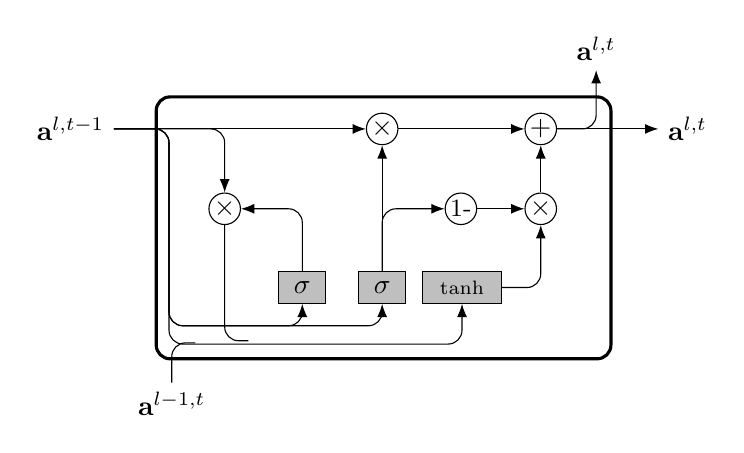
\begin{tikzpicture}[
		scalar/.style={circle, draw, inner sep=0pt, minimum width=4mm},
		tanlayer/.style={rectangle, draw, inner sep=0pt, fill=gray!50, minimum width=10mm, minimum height=4mm},
		siglayer/.style={rectangle, draw, inner sep=0pt, fill=gray!50, minimum width=6mm, minimum height=4mm},
		textb/.style={minimum width=6mm, minimum height=4mm},
		ct/.style={circle, draw, inner sep=5pt, ultra thick, minimum width=10mm},
		ft/.style={circle, draw, minimum width=8mm, inner sep=1pt},
		filter/.style={circle, draw, minimum width=7mm, inner sep=1pt, path picture={\draw[thick, rounded corners] (path picture bounding box.center)--++(65:2mm)--++(0:1mm);
		\draw[thick, rounded corners] (path picture bounding box.center)--++(245:2mm)--++(180:1mm);}},
		mylabel/.style={font=\scriptsize\sffamily},
		>=LaTeX
	]
	
	\node[scalar] (times) {$\times$};
	\node[scalar, right=16mm of times] (plus) {$+$};
	\node[scalar, below=6mm of plus] (times2) {$\times$};
	\node[scalar, left=6mm of times2] (minus1) {\small 1-};
	\node[scalar, left=36mm of times2] (times3) {$\times$};
	\node[siglayer, below=16mm of times] (sig2) {$\sigma$};
	\node[siglayer, left=4mm of sig2] (sig1) {$\sigma$};
	\node[tanlayer, right=2mm of sig2] (tanh) {\scriptsize $\tanh$};
	\node[textb, anchor=east, left=32mm of times] (hin) {$\mathbf{a}^{l, t - 1}$};
	\node[textb, anchor=west, right=33mm of times] (hout) {$\mathbf{a}^{l, t}$};
	\node[textb, anchor=north, below left=10mm and 8mm of sig1] (x) {$\mathbf{a}^{l - 1, t}$};
	\node[textb, anchor=south, above right=6mm and 22mm of times] (hout2) {$\mathbf{a}^{l, t}$};
	\node[below right=2.5mm and 17.5mm of sig2] (invisible) {};
	\node[left=7mm of sig1] (invisible2) {};
	\node[fit=(plus) (tanh) (invisible) (invisible2), draw, inner xsep=6mm, inner ysep=2mm, rounded corners=5pt, line width=0.4mm] (fit) {};

	\foreach \i/\j in {hin/times3, plus/hout2, tanh/times2}
		\draw[->, rounded corners=5pt] (\i) -| (\j);

	\foreach \i/\j in {sig1/times3, sig2/minus1}
		\draw[->, rounded corners=5pt] (\i) |- (\j);

	\foreach \i/\j in {hin/times, times/plus, plus/hout, times2/plus, minus1/times2, sig2/times}
		\draw[->] (\i) -- (\j);

	\foreach \i/\j in {hin.east/sig1.south, hin.east/sig2.south}
		\draw[->, rounded corners=5pt] (\i) -| ++(7mm,-25mm) -| (\j);
		
	\draw[->, rounded corners=5pt] (hin.east) -| ++(7mm,-27.32mm) -| (tanh.south);

	\draw[-, rounded corners=5pt] (times3.south) |- ++(3mm, -14.69mm);

	\draw[-, rounded corners=5pt] (x.north) |- ++(3mm, 5.045mm);

	\end{tikzpicture}}
	\caption{A GRU cell.}
\end{subfigure}
\caption{Various architectures of RNN neurons, using the notation from figure~\ref{fig:rnn_notation}}
\end{figure}

\subsection{Word Embeddings} \label{word_embeddings}

RNNs take a sequence of vectors as input, and produce a sequence of vectors as output. In the context of language modelling, these inputs and outputs should represent sequences of words. In order to do this, each word is represented by a single vector, which is known as a word \tit{embedding}. \\

The aim behind word embeddings is that similar words should be represented by vectors that are closer together in the vector space than those for dissimilar words. One effective way to obtain such embeddings is to learn them through backpropagation, which is the method that was used in this dissertation. The idea is that each word is mapped to a large, randomly initialised vector. Then, when the RNN is trained on sequences of words, the embedding values are updated in a way that is analogous to how the weights are updated in the network.

\section{Software Engineering}

In this section details the requirements of the project and the early design decisions that were made to target those goals.

\subsection{Requirements}

The success requirements set out in the project proposal were:

\begin{center}
\begin{tabular}{L{1cm} L{14cm}}
	\hline
	\tbf{R1} & Language models (LMs) using the following techniques are implemented:
	\begin{itemize}[nosep]
	\item
		$n$-gram LMs with various smoothing techniques.
	\item
		A vanilla RNN-based LM.
	\item
		An LSTM-based LM.
	\end{itemize}\\[-\normalbaselineskip] \hline
	\tbf{R2} & Comprehensible and reliable comparisons between the various LM implementations and their combinations are made regarding their accuracy, speed and resource consumption during both training and inference. \\ \hline
	\tbf{R3} & A simple console application is developed to demonstrate the capability of the aforementioned language models in the context of next-word prediction. \\ \hline
\end{tabular}
\end{center}

The project proposal also suggested two possible extensions:
\begin{center}
\begin{tabular}{L{1cm} L{14cm}}
	\hline
	\tbf{E1} & Explore possible extensions to existing language models to improve their performance on error-prone text. \\ \hline
	\tbf{E2} & Build a mobile keyboard that exhibits the functionality of the language models. \\ \hline
\end{tabular}
\end{center}

All requirements and extensions depend on \tbf{R1}, so I implemented that first. Afterwards, I built \tbf{R2} and \tbf{R3} in parallel before moving onto \tbf{E1} and \tbf{E2}.

\subsection{Tools and Technologies Used} \label{tools}

Below I describe and justify where necessary the tools and technologies that I selected to build my project.

\subsubsection{Version Control and Build Tools}

I hosted my project in a repository on GitHub, used Git for version control, and used Bazel for running builds and tests on my project.

\subsubsection{Machine Learning}

I chose to use TensorFlow, an open source machine learning library, to assist in the implementation of my recurrent neural networks. There are two key reasons for this:
\begin{enumerate}
\item
	TensorFlow supports \tit{automatic differentiation}. That is, each tensor operation has a partial derivative associated with it, so when you want to apply the second stage of backpropagation, TensorFlow can automatically apply the chain rule through any sequence of tensor operations. Without this, I would have to hard-code new gradient calculations every time I change the structure of the network, which is tedious and error-prone.
\item
	TensorFlow supports GPU-accelerated matrix operations. Without this, training my recurrent neural networks would take significantly longer.
\end{enumerate}
Of course, there are many other machine learning libraries that offer comparable features. The reason I picked TensorFlow in particular was because I was already familiar with its codebase from using and contributing to it during an internship at Google in 2016. \\

In order to train large scale models on NVIDIA GPUs, I used the University's High Performance Computing service.

\subsubsection{Languages}

At the time of writing my code, TensorFlow had both a C++ and a Python API. However, the C++ API only had support for loading and running inference on models, not for training them. \\

One of the possible extensions I set out in my project proposal was to implement a mobile keyboard that makes use of my language model implementations. Android and iOS both provide little or no support for applications written in Python, but they do support code written in C++ via the JNI and Objective-C++ respectively. \\

I used C++ to write the benchmarking framework and all $n$-gram language models, so that they could easily be used within a mobile application. As for the RNN-based language models, I wrote code to train and export them in Python, and then wrote some C++ classes for loading and running inference on them. This way, I could leverage the power of TensorFlow's Python API whilst also supporting the use of such models in a mobile keyboard. In order to export and import trained language models across different languages, I used Google's protocol buffers, a language neutral mechanism for serialising structured data.

\subsubsection{Testing}

I used Google Test for C++ unit tests and the \ttt{unittest} package for testing in Python.

\subsection{Starting Point}

My project codebase was written from scratch, with the assistance of the tools and libraries mentioned in section \ref{tools}. Before the project, I had no understanding of language modelling. Apart from a basic knowledge of recurrent neural networks, I had to learn about language modelling, $n$-gram smoothing techniques, long short-term memory and gated recurrent units through personal reading. \\

\begin{figure}[h]
\captionsetup{justification=centering}
\centering
\begin{tabular}{| l | l |}
	\hline
	\tbf{Experience} & \tbf{Tools and Technologies} \\ \hline
	\tit{Significant} & C++, Python, Git, GitHub, TensorFlow \\
	\tit{Some} & Bazel, iOS, Protocol Buffers \\
	\tit{None} & Google Test, Objective-C++, SLURM \\ \hline
\end{tabular}
\caption{A summary of my prior experience with the tools and technologies used in this project.}
\end{figure}

\chapter{Implementation} \label{implementation}

This section details how I implemented a variety $n$-gram and RNN-based language models, how I built the mobile keyboard on iOS and how I extended an existing language model to improve its performance on error-prone text.

\section{System Overview}

\tikzstyle{vecArrow} = [thick, decoration={markings,mark=at position
	1 with {\arrow[semithick]{open triangle 60}}},
	double distance=1.4pt, shorten >= 5.5pt,
	preaction = {decorate},
	postaction = {draw,line width=1.4pt, white,shorten >= 4.5pt}]

\begin{figure}[h]
\captionsetup{justification=centering}
\begin{adjustbox}{center}
\centering
\begin{tikzpicture}[
		>=stealth,
		language/.style={rectangle, rounded corners=5pt},
		module/.style={draw, rectangle, thick, rounded corners=2pt, minimum width=25mm, minimum height=15mm, text width=25mm, align=center},
	]
	\node[language, minimum width=60mm, minimum height=30mm, fill=purple!10] (objectiveC) at (-5.5, 0) {};
	\node[language, minimum width=60mm, minimum height=30mm, fill=brown!10] (python) at (-5.5, -4) {};
	\node[language, minimum width=170mm, minimum height=30mm, fill=black!10] (protobuf) at (0, -8) {};
	\node[language, minimum width=100mm, minimum height=70mm, fill=blue!10] (cplusplus) at (3.5, -2) {};
	
	\node[below right] (objectiveC_text) at (objectiveC.north west) {\tbf{Objective-C++}};
	\node[below right] (python_text) at (python.north west) {\tbf{Python}};
	\node[below right] (protobuf_text) at (protobuf.north west) {\tbf{Protocol Buffer}};
	\node[below right] (cplusplus_text) at (cplusplus.north west) {\tbf{C++}};

	\node[module, below right=7.5mm and 15mm, dashed] (mobile_keyboard) at (objectiveC.north west) {\footnotesize iOS Mobile Keyboard};

	\node[module, below right=7.5mm and 15mm] (rnn_train) at (python.north west) {\footnotesize RNN LM Training};

	\node[module, below right=7.5mm and 51mm] (rnn_proto) at (protobuf.north west) {\footnotesize Trained RNN LM};
	\node[module, below right=7.5mm and 85mm] (ngram_proto) at (protobuf.north west) {\footnotesize Trained $n$-gram LM};

	\node[module, below right=7.5mm and 15mm] (benchmark) at (cplusplus.north west) {\footnotesize Benchmarking Framework};
	\node[module, below right=25mm and 11.5mm, minimum width=75mm, minimum height=40mm] (lm) at (cplusplus.north west) {};
	\node[module, below right=27.5mm and 15mm] (rnn_infer) at (cplusplus.north west) {\footnotesize RNN LM Inference};
	\node[module, below right=27.5mm and 55mm, dashed] (error_correcting) at (cplusplus.north west) {\footnotesize Error-Correcting RNN LM};
	\node[module, below right=47.5mm and 15mm] (ngram) at (cplusplus.north west) {\footnotesize $n$-gram LM Training / Inference};
	\node[module, below right=47.5mm and 55mm] (combination) at (cplusplus.north west) {\footnotesize Combined LM};

	\foreach \i/\j in {error_correcting/rnn_infer, combination/ngram, combination/rnn_infer}
		\draw[->] (\i) -- (\j);

	\draw[->, rounded corners=5pt] (mobile_keyboard.east) -| ++(22.5mm,-10mm) |- ([yshift=2mm]rnn_infer.west);

	\draw[->, rounded corners=5pt] (benchmark) -| (lm);

	\draw[vecArrow, rounded corners=5pt] (rnn_train.east) -| ([xshift=-2mm]rnn_proto.north);
	\draw[vecArrow, rounded corners=5pt] ([xshift=2mm]rnn_proto.north) |- ([yshift=-2mm]rnn_infer.west);

	\draw[vecArrow, rounded corners=5pt] ([xshift=-2mm]ngram.south) -- ([xshift=-2mm]ngram_proto.north);
	\draw[vecArrow, rounded corners=5pt] ([xshift=2mm]ngram_proto.north) -- ([xshift=2mm]ngram.south);

\end{tikzpicture}
\end{adjustbox}
\caption{An overview of the project. Outlined rectangles denote groups of related files or code, of which the ones with a dashed outline represent project extensions. Thin arrows denote dependencies and thick arrows represent the movement of data.}
\label{fig:system_overview}
\end{figure}

The core components of my project are highlighted in figure~\ref{fig:system_overview}. The choices of language for each of the system components are reasoned in section~\ref{tools}. I used Protocol Buffers as a language neutral method of encapsulating a trained and exported language model that can be loaded into memory and used to make predictions. \\

As shown, all of the code for training and running inference on $n$-gram models was written in C++, and is described in section~\ref{ngram_lm}. The RNN-based language models were trained in Python using TensorFlow, before being exported into a small group of protocol buffers that can be loaded into C++ for running inference, all of which is detailed in section~\ref{rnn_lm}. The `Combined LM' component represents a language model which interpolates the probabilities across one or more $n$-gram and/or RNN-based language models. This part is not described in depth, because it is mostly trivial. I outline in section~\ref{mobile_keyboard} how I built a mobile keyboard in iOS that utilises one of the RNN-based language models. Finally, the `Error-Correcting RNN LM' component denotes an extension to an existing RNN-based language model which I made in order to improve its performance on error-prone text, which is described in section~\ref{error_correcting_lm}. \\

The $n$-gram, RNN, error-correcting RNN and combined language models all inherit, either directly or indirectly, from a single language model superclass, which is all that the benchmarking framework depends on. This class is described briefly below. Details of the metrics used in the benchmarking framework are left for chapter~\ref{evaluation}. \\

\subsection{The Language Model Hierarchy} \label{lm_interface}

All of my language model implementations in C++ were joined by the same inheritance hierarchy, at the top of which was a single language model superclass, \ttt{LM}: \\

\begin{lstlisting}[language=C++]
class LM {
protected:
    Vocab *vocab;
    ...
public:
    ...
    // Given a sequence of words, `seq', return the most probable next word, with its
    // associated probability.
    virtual void Predict(std::list<std::string> seq,
                         std::pair<std::string, double> &pred);
    
    // Given a sequence of words, `seq', return the top k most probable next words, in
    // order of decreasing probability.
    virtual void PredictTopK(std::list<std::string> seq,
                             std::list<std::pair<std::string, double>> &preds, int k);
    
    // Return the probability of the word sequence, `seq'.
    virtual double Prob (std::list<std::string> seq) = 0;
    
    // Given a sequence of words, `seq', initialise `probs' with the probability of each
    // word in the vocabulary following that sequence.
    virtual void ProbAllFollowing (std::list<std::string> seq,
                                   std::list<std::pair<std::string, double>> &probs) = 0;
    
    // The same as above, except the word-probabilities are stored in a character trie.
    virtual void ProbAllFollowing (std::list<std::string> seq, CharTrie *probs) = 0;
    ...
};
\end{lstlisting}
~\\

Every language model object stores a \ttt{Vocab} object, which contains the set of words in the language model vocabulary, and a mapping from those words to integer IDs. The integer IDs are used in place of the string representations of such words in various language model data structures that are discussed later in this chapter. This is simply a memory optimisation, because an integer requires less space than a string. \\

\ttt{Predict()} is a special case of \ttt{PredictTopK()}, which simply uses a priority queue to extract the top $k$ predictions from result of calling \ttt{ProbAllFollowing()}. The implementations of \ttt{Prob()} and \ttt{ProbAllFollowing()} depend on the specific language model. One might think that \ttt{ProbAllFollowing()} can be implemented by calling \ttt{Prob()} for each word in the vocabulary, but this would be inefficient in the case of an RNN-based language model, which implicitly computes the probability distribution over every word in the vocabulary in each forward pass of the network, hence why the methods are kept separate. \\

\todo{Possibly add diagram of inheritance hierarchy.}

\section{$n$-gram Models} \label{ngram_lm}

Below I detail the implementation of the $n$-gram models and their associated smoothing techniques. \\

One of the first things I discovered when implementing $n$-gram language models is that there is a tradeoff between how much computation is done at training time, and how much computation is done at inference time. For example, at one extreme you could compute only the number of times each $n$-gram occurs at training time, and leave the computation of the coefficients in the smoothing equations to be calculated on the fly. At the other extreme, you could compute and store the final value of the probability for every possible $n$-gram that can be formed from the words in the language model vocabulary, and then return the relevant probability immediately at inference time. The problem with the first approach is that the language model would be too slow at inference time, and the problem with the second approach is that storing absolute probabilities for every possible $n$-gram would occupy far too much space to be practical. In my implementation, I try to strike a balance between these two extremes by precomputing and efficiently storing all of the relevant coefficients for the smoothing equations, and then combining them at inference time to compute the required $n$-gram probability. \\

\begin{figure}[h]
\captionsetup{justification=centering}
\centering
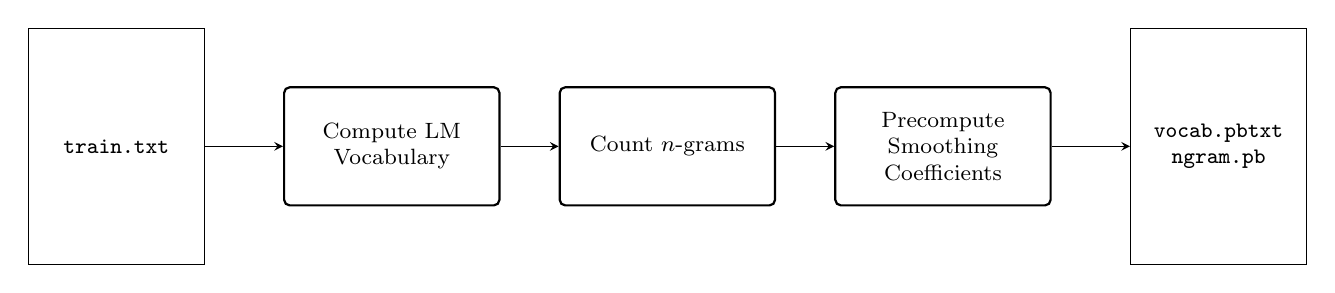
\begin{tikzpicture}[
		>=stealth,
		stage/.style={draw, rectangle, thick, rounded corners=2pt, minimum width=25mm, minimum height=15mm, text width=25mm, align=center, font=\footnotesize},
		file/.style={draw, rectangle, minimum width=20mm, minimum height=30mm, text width=20mm, align=center, font=\footnotesize\ttfamily},
	]
	\node[file] (training_set) at (0, 0) {\ttt{train.txt}};
	\node[stage] (vocab) at (3.5, 0) {Compute LM Vocabulary};
	\node[stage] (count) at (7, 0) {Count $n$-grams};
	\node[stage] (precompute) at (10.5, 0) {Precompute Smoothing Coefficients};
	\node[file] (ngram_proto) at (14, 0) {vocab.pbtxt \\ ngram.pb};

	\draw[->] (training_set) -- (vocab);
	\draw[->] (vocab) -- (count);
	\draw[->] (count) -- (precompute);
	\draw[->] (precompute) -- (ngram_proto);
\end{tikzpicture}
\caption{The $n$-gram training pipeline.}
\label{fig:ngram_training}
\end{figure}

The process of training an $n$-gram model in my implementation is outlined in figure~\ref{fig:ngram_training}. The three stages of the pipeline are outlined in sections~\ref{ngram_compute_vocab}, \ref{ngram_count} and \ref{ngram_precompute} respectively.

\subsection{Computing the Vocabulary} \label{ngram_compute_vocab}

The first stage involves a single pass over \ttt{train.txt}, where words that occur at least $k$ times are added to the vocabulary and mapped to an integer ID. A special marker \ttt{<unk>} is included in the vocabulary to represent any out-of-vocabulary words. That is, when the model encounters a word it has not seen before, it treats it as \ttt{<unk>}. The marker \ttt{<s>} is also included and is used to denote the end of a sentence.

\subsection{Counting $n$-grams Efficiently} \label{ngram_count}

For $n$-gram models without any smoothing, the only information that needs to be computed at this stage is $c(w_{i - n + 1}^{i})$ and $\sum_w c(w_{i - n + 1}^{i - 1}w)$, which are the number of times each $n$-gram $w_{i - n + 1}^i$ occurred in \ttt{train.txt}, and the sum of all such counts that follow the $(n-1)$-gram $w_{i - n + 1}^{i - 1}$ respectively. Then, given these two precomputed numbers, when the $n$-gram model is queried for the probability of $w_{i - n + 1}^i$, it can simply return the first number divided by the second, as required in equation~\ref{eq:ngram}. \\

This situation becomes more complex once smoothing techniques are included.

\begin{itemize}
\item
	Count trie
	\begin{itemize}
	\item
		Interface
	\item
		Efficient count following/preceding
	\item
		Efficient sum following
	\end{itemize}
\end{itemize}
\subsection{Precomputing Smoothing Coefficients} \label{ngram_precompute}
\begin{itemize}
\item
	How all smoothing methods can be massaged to same form, which suits storage in probability trie.
\item
	Probability trie - explain how it stores each parameter the minimum number of times.
\end{itemize}
\section{Recurrent Neural Network Models} \label{rnn_lm}
\subsection{TensorFlow}
\begin{itemize}
\item
	How it works
\item
	Training vs inference flow
\end{itemize}
\subsection{Long Short-Term Memory}
\begin{itemize}
\item
	Forward pass equations
\item
	Explain gates
\item
	Dropout, embedding, learning rate decay, momentum?, gradient clipping
\end{itemize}
\subsection{Gated Recurrent Units}
\begin{itemize}
\item
	Explain
\end{itemize}
\subsection{Word Embeddings}
\begin{itemize}
\item
	PCA plots
\end{itemize}
\subsection{Parameter Tuning}
\begin{itemize}
\item
	Learning rate schedule using validation set, initial learning rate, dropout, etc
\end{itemize}

\section{Mobile Keyboard} \label{mobile_keyboard}
\begin{itemize}
\item
	Compiling my project, along with TensorFlow into a static library for use on iOS.
\end{itemize}
\subsection{Updating Language Model Predictions On the Fly}
\begin{itemize}
\item
	Building a character trie when a new word is requested, sifting through it as new characters are typed
\item
	Screenshots
\end{itemize}

\section{Extending Models to Tackle Error-Prone Text} \label{error_correcting_lm}
\subsection{Preprocessing the CLC Dataset}
\begin{itemize}
\item
	Tokenisation
\item
	Alignment and removal of identical sentences
\end{itemize}
\subsection{Error Correction on Word Context}
\begin{itemize}
\item
	Motivation and algorithm for error-correction on the context
\end{itemize}

\chapter{Evaluation} \label{evaluation}

In this chapter, I will first describe the benchmarking framework that I built to evaluate the language models, before proceeding onto the results. The results section is threefold: firstly I present the performance of the existing language models that I implemented, secondly I focus on the tradeoffs faced when employing those models on a mobile device, and finally I display my findings in language modelling on error-prone text.

\todo{Include these too:}
\begin{itemize}
\item
	Examples of generated sentences.
\item
	Visualisations of the neuron activations for each word in a sentence.
\end{itemize}

\section{Evaluation Methodology}

\subsection{Metrics} \label{metrics}

In the context of text prediction, there are essentially two questions one might want to answer when evaluating a language model:
\begin{enumerate}
\item
	How accurately does the language model predict text?
\item
	How much resource, such as CPU or memory, does the language model consume?
\end{enumerate}

In order to answer these questions, I implemented a generic benchmarking framework that can return a series of metrics that fall into one of the two aforementioned categories when given a language model. These metrics include perplexity, average-keys-saved, memory usage and average inference time. The first two are concerned with the accuracy of language models and the latter two relate to the resource usage. I also recorded how long it took to train each model.

\subsubsection{Perplexity}

Perplexity is the most widely-used metric for language models, and is therefore an essential one to include so that my results can be compared with those of other authors. Given a sequence of words $w_1^{N} = w_1w_2...w_N$ as test data, the perplexity PP of a language model $L$ is defined as:
\begin{gather} \label{eq:perplexity}
	\text{PP}_L(w_1^N) = \sqrt[N]{\frac{1}{\mathbb{P}_L(w_1^N)}} = \sqrt[N]{\prod_{i=1}^{N}\frac{1}{\mathbb{P}_L(w_i | w_1^{i-1})}}
\end{gather}
where $\mathbb{P}_L(w_i | w_1^{i-1})$ is the probability computed by the language model $L$ of the word $w_i$ following the words $w_1^{i-1}$. The key point is that \tbf{lower values of perplexity indicate better prediction accuracy} for language models trained on a particular training set. \\

This somewhat arbitrary-looking formulation can be better understood from a touch of information theory. In information theory, the cross-entropy $H(p, q)$ between a true probability distribution $p$ and an estimate of that distribution $q$ is defined as:\footnote{Note that $H(p, q)$ is often also used to denote the joint entropy of $p$ and $q$, which is a different concept.}
\begin{gather*}
	H(p, q) = -\sum_x p(x) \log_2 q(x)
\end{gather*}
It can be shown that $H(p, q) = H(p) + D_{KL}(p || q)$ where $D_{KL}(p || q) \geq 0$ is the Kullback-Leibler distance between $p$ and $q$. Generally speaking, the better an estimate $q$ is of $p$, the lower $H(p, q)$ will be, with a lower bound of $H(p)$, the entropy of $p$. \\

The perplexity PP of a model $q$, with respect to the true distribution $p$ it is attempting to estimate, is defined as:
\begin{gather} \label{eq:perplexity_to_cross_entropy}
	\text{PP} = 2^{H(p, q)}
\end{gather}

Language models assign probability distributions over sequences of words, and so it seems reasonable to use perplexity as a motivation for a measure of their performance. In the context of language modelling, however, we do not know what the underlying distribution of $p$ is, so it is approximated with Monte Carlo estimation by taking samples of $p$ (i.e. sequences of words from the test data) as follows:
\begin{gather*}
	\text{PP}_L(w_1^N) = 2^{-\frac{1}{N}\sum_i \log_2 \mathbb{P}_L(w_i | w_1^{i-1})}
\end{gather*}
With a little algebra, this can be rearranged to give equation~\ref{eq:perplexity}. \\

One issue with perplexity is that it is undefined if $\mathbb{P}_L(w_i | w_1^{i-1})$ is 0 at any point. To get around this in my implementation, I replaced probability values of 0 with the small constant \ttt{1e-9}. Results that use this approximation are marked.

\subsubsection{Average-Keys-Saved}

It is typical for the top three next-word predictions to be displayed and updated as the user types in a mobile keyboard, as described in section~\ref{mobile_keyboard}. Clearly, it is in the interest of the mobile keyboard developer to minimise the amount of typing a user has to do before the correct prediction is displayed. Average-keys-saved is based on this incentive, and is defined as the number of keys that the user would be saved from typing as a result of the correct next word appearing in the top three predictions, averaged over the number of characters in the test data. \\

As an example, if the user is typing \ttt{science} and the word \ttt{science} appears in the top three predictions after they have typed \ttt{sc}, then that would count as 5 characters being saved, averaging at $\frac{5}{7}$ keys saved per character. Averaging over the number of characters in the test data ensures that the results are not biased by the data containing particularly long words, which are easier to save characters on.

\subsubsection{Memory Usage}

This is measured as the amount of physical memory in megabytes occupied by the process in which the language model under test is instantiated.

\subsubsection{Training Time}

The amount of time it took to train the language model.

\subsubsection{Average Inference Time}

This is measured as the amount of time in milliseconds that the language model takes to assign a probability to all of the words in its vocabulary given a sequence of words, averaged over a large number of sequences.

\subsection{Datasets}

I used three datasets throughout the evaluation of my project:

\subsubsection{Penn Tree Bank (PTB) Dataset}

The Penn Tree Bank is a popular dataset for measuring the quality of language models, created from text from the Wall Street Journal. It has already been preprocessed such that numbers are replaced with \ttt{N}, rare words are replaced with \ttt{<unk>} and the text has been split up into one sentence per line. It has been split up into a training, validation and test set. The training set has 10,000 unique words and 887,521 words overall. \\

Given that the Penn Tree Bank is so widely adopted, I used it for all tests in which the size of the training data is fixed, and will refer to it as PTB.

\subsubsection{One Billion Word (1BW) Benchmark}

This is a much larger dataset produced by Google of approximately 1 billion words~\cite{1bw:chelba2013}. I used this dataset for tests in which the size of the training data is a variable under investigation, and will refer to it as 1BW.

\subsubsection{Cambridge Learner Corpus (CLC)}

The Cambridge Learner Corpus is a dataset of 1,244 exam scripts written by candidates sitting the Cambridge ESOL First Certificate in English (FCE) examination in 2000 and 2001~\cite{clc:yannakoudakis2011}. The original dataset contains the scripts annotated with corrections to all of the mistakes by the candidates. In this project I make use of a preprocessed version of the dataset, in which there is one file containing the error-free version of the exam scripts and there is another file containing the original exam scripts with their errors. These two files are aligned line by line. I used this dataset when exploring the performance of language models on error-prone text, and will refer to it as CLC.

\section{Results}

\subsection{Existing Models}

\subsubsection*{Smoothing techniques and the value of $n$ in $n$-gram models}

The first set of language models that I built were $n$-gram models, along with a series of smoothing techniques for improving their predictions on less frequent $n$-grams.

\begin{figure}[h]
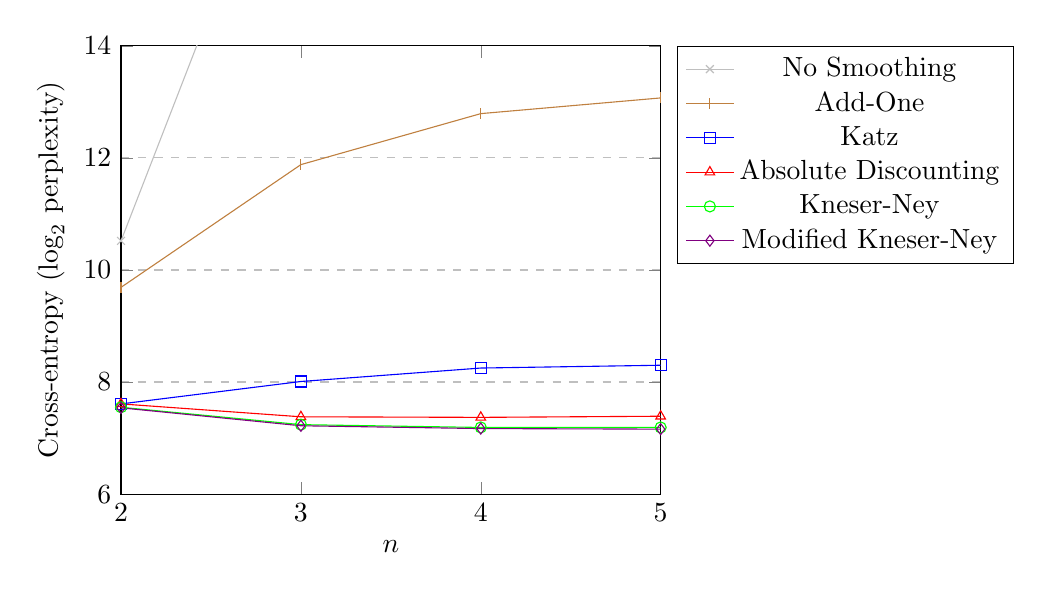
\begin{tikzpicture}[scale=1.0]
\begin{axis}[
	xlabel={$n$},
	ylabel={Cross-entropy ($\log_2$ perplexity)},
	xmin=2, xmax=5,
	ymin=6, ymax=14,
	xtick={2, 3, 4, 5},
	ytick={6, 8, 10, 12, 14},
	legend pos=outer north east,
	ymajorgrids=true,
	grid style=dashed,
]

\addplot[color=lightgray, mark=x]
coordinates {(2, 10.52)(3, 18.79)(4, 24.95)(5, 27.55)};

\addplot[color=brown, mark=|]
coordinates {(2, 9.69)(3, 11.88)(4, 12.79)(5, 13.07)};

\addplot[color=blue, mark=square]
coordinates {(2, 7.61)(3, 8.01)(4, 8.25)(5, 8.30)};

\addplot[color=red, mark=triangle]
coordinates {(2, 7.61)(3, 7.38)(4, 7.37)(5, 7.39)};

\addplot[color=green, mark=o]
coordinates {(2, 7.55)(3, 7.24)(4, 7.19)(5, 7.19)};

\addplot[color=violet, mark=diamond]
coordinates {(2, 7.54)(3, 7.22)(4, 7.17)(5, 7.16)};

\legend{No Smoothing, Add-One, Katz, Absolute Discounting, Kneser-Ney, Modified Kneser-Ney}
 
\end{axis}
\end{tikzpicture}
\caption{Cross-entropy of $n$-gram models trained on the PTB dataset.}
\end{figure}

Recall from equation~\ref{eq:perplexity_to_cross_entropy} that cross-entropy is just the binary logarithm of perplexity, and that lower perplexity scores indicate better prediction accuracy. With this in mind, it is clear that modified Kneser-Ney smoothing offers the best prediction performance amongst the $n$-gram models. \\

The change in performance with the value of $n$ is interesting. Intuitively, one might expect that increasing $n$ will always yield better results, because this corresponds to increasing the number of words you use to make a prediction. However, for $n$-gram models with no smoothing, add-one smoothing or Katz smoothing, this is not the case. For $n$-gram models with add-one or no smoothing, this is because they do not employ backoff. At higher values of $n$, $n$-grams are much more sparse, so without any backoff higher $n$-gram models can only rely on sparse counts, resulting is lower probabilities being assigned to plausible sequences of words. Katz smoothing does employ backoff, and achieves much better performance, but it still distributes too much probability to rare $n$-grams.

\subsubsection*{A comparison of RNN-based models with $n$-gram models}

As described in the implementation chapter, I also implemented three RNN-based language models which differ in the RNN cell architecture: vanilla RNN, Gated Recurrent Unit and Long Short-Term Memory. \\

\begin{figure}[h]
\captionsetup{justification=centering}
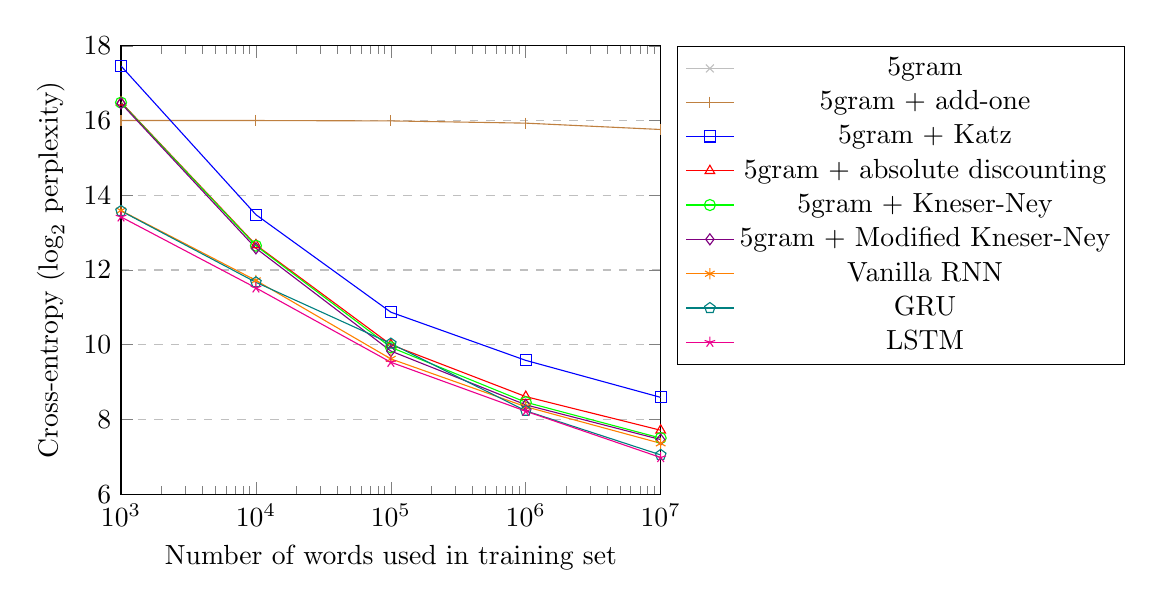
\begin{tikzpicture}[scale=1.0]
\begin{semilogxaxis}[
	xlabel={Number of words used in training set},
	ylabel={Cross-entropy ($\log_2$ perplexity)},
	xmin=1e3, xmax=1e7,
	ymin=6, ymax=18,
	legend pos=outer north east,
	ymajorgrids=true,
	grid style=dashed,
]

% 3gram
%\addplot[color=lightgray, mark=x]
%coordinates {(1e3, 29.33)(1e4, 28.22)(1e5, 25.58)(1e6, 21.29)(1e7, 16.25)};

% 3gram + add-one
%\addplot[color=brown, mark=|]
%coordinates {(1e3, 15.97)(1e4, 15.87)(1e5, 15.59)(1e6, 14.93)(1e7, 13.77)};

% 3gram + Katz
%\addplot[color=blue, mark=square]
%coordinates {(1e3, 17.40)(1e4, 13.48)(1e5, 10.83)(1e6, 9.28)(1e7, 8.14)};

% 3gram + absolute discounting
%\addplot[color=red, mark=triangle]
%coordinates {(1e3, 16.46)(1e4, 12.61)(1e5, 9.92)(1e6, 8.54)(1e7, 7.68)};

% 3gram + Kneser-Ney
%\addplot[color=green, mark=o]
%coordinates {(1e3, 16.45)(1e4, 12.60)(1e5, 9.85)(1e6, 8.41)(1e7, 7.54)};

% 3gram + modified Kneser-Ney
%\addplot[color=violet, mark=diamond]
%coordinates {(1e3, 16.46)(1e4, 12.58)(1e5, 9.84)(1e6, 8.40)(1e7, 7.53)};

% 5gram
\addplot[color=lightgray, mark=x]
coordinates {(1e3, 29.89)(1e4, 29.83)(1e5, 29.58)(1e6, 28.86)(1e7, 27.10)};

% 5gram + add-one
\addplot[color=brown, mark=|]
coordinates {(1e3, 16.00)(1e4, 16.00)(1e5, 15.99)(1e6, 15.93)(1e7, 15.76)};

% 5gram + Katz
\addplot[color=blue, mark=square]
coordinates {(1e3, 17.46)(1e4, 13.48)(1e5, 10.87)(1e6, 9.58)(1e7, 8.59)};

% 5gram + absolute discounting
\addplot[color=red, mark=triangle]
coordinates {(1e3, 16.49)(1e4, 12.67)(1e5, 10.00)(1e6, 8.61)(1e7, 7.71)};

% 5gram + Kneser-Ney
\addplot[color=green, mark=o]
coordinates {(1e3, 16.48)(1e4, 12.65)(1e5, 9.93)(1e6, 8.46)(1e7, 7.50)};

% 5gram + modified Kneser-Ney
\addplot[color=violet, mark=diamond]
coordinates {(1e3, 16.46)(1e4, 12.58)(1e5, 9.83)(1e6, 8.39)(1e7, 7.46)};

% Vanilla RNN 256
\addplot[color=orange, mark=asterisk]
coordinates {(1e3, 13.59)(1e4, 11.72)(1e5, 9.62)(1e6, 8.34)(1e7, 7.36)};

% GRU 256
\addplot[color=teal, mark=pentagon]
coordinates {(1e3, 13.58)(1e4, 11.67)(1e5, 10.03)(1e6, 8.23)(1e7, 7.05)};

% LSTM 256
\addplot[color=magenta, mark=star]
coordinates {(1e3, 13.42)(1e4, 11.52)(1e5, 9.53)(1e6, 8.22)(1e7, 6.98)};

\legend{
%	3gram, 3gram + add-one, 3gram + Katz, 3gram + absolute discounting, 3gram + Kneser-Ney, 3gram + Modified Kneser-Ney,
	5gram, 5gram + add-one, 5gram + Katz, 5gram + absolute discounting, 5gram + Kneser-Ney, 5gram + Modified Kneser-Ney,
	Vanilla RNN, GRU, LSTM,
}
 
\end{semilogxaxis}
\end{tikzpicture}
\caption{Cross-entropy of various language models with respect to the training set size, using the 1BW dataset.}
\label{fig:cross_entropy_training_set_size}
\end{figure}

As can be seen in figure~\ref{fig:cross_entropy_training_set_size}, the RNN-based language models consistently outperform the $n$-gram based models in terms of prediction accuracy. This difference is most significant for small training sets of less than $10^5$ words, and starts to become more pronounced again once the training set grows large beyond $10^6$ words. The performance gain from adding more training data seems to start flattening out towards $10^7$ words for the smoothed $n$-gram models, whereas the RNN-based ones seem to continue improving. \\

Some datasets are more predictable than others, which means that metrics like perplexity and average-keys-saved depend on which dataset is used. In order to produce metrics that are comparable with the work of other authors, I have tested my language models on the Penn Tree Bank dataset, as shown in figure~\ref{fig:ptb}. The perplexity was calculated over the whole of the test set, whereas average-keys-saved, a more expensive metric to compute, was taken over the first 1000 words of the test set. Indeed, my results for 3-gram modified Kneser-Ney smoothing, 5-gram modified Kneser-Ney smoothing and the vanilla RNN are comparable to those from Mikolov~\cite{rnn_ptb:mikolov2012}, who also benchmarked these three models. \\

\begin{figure}[h]
\begin{adjustbox}{center}
\begin{tabular}{| L{5.2cm} | C{2.2cm} | C{2cm} | C{2cm} |  C{2cm} | C{2cm} |}
	\hline
	\tbf{Language Model} & \tbf{Perplexity} & \tbf{Average-Keys-Saved} & \tbf{Memory Usage (MB)} & \tbf{Training Time (min,secs)}$^\dagger$ & \tbf{Average Inference Time (ms)} \\ \hline
	3-gram & 4.54 $\times 10^5$$^*$ & 0.35014 & 266.91 & \tbf{11s} & 62 \\
	3-gram + add-one & 3764.96 & 0.53063 & 266.94 & \tbf{11s} & 41 \\
	3-gram + Katz & 256.95 & 0.68482 & 266.71 & 14s & 88 \\
	3-gram + absolute disc. & 166.03 & 0.72178 & 266.78 & 13s & 63 \\
	3-gram + KN & 150.73 & 0.72466 & 266.88 & 14s & 54 \\
	3-gram + modified KN & 149.54 & 0.72355 & 266.97 & 14s & 54 \\
	5-gram & 1.96 $\times 10^8$$^*$ & 0.07167 & 737.36 & 26s & 130 \\
	5-gram + add-one & 8610.45 & 0.33886 & 737.30 & 26s & 63 \\
	5-gram + Katz & 314.49 & 0.67154 & 737.43 & 41s & 156 \\
	5-gram + absolute disc. & 167.38 & 0.72333 & 737.43 & 40s & 126 \\
	5-gram + KN & 146.35 & 0.72598 & 737.37 & 44s & 114 \\
	5-gram + modified KN & 142.68 & 0.72554 & 737.53 & 50s & 116 \\ \hline
	Vanilla RNN & 131.03 & 0.72776 & \tbf{253.67} & 15m 10s & 39 \\
	Gated Recurrent Units & 114.52 & 0.73993 & 271.39 & 28m 35s & \tbf{37} \\
	Long Short-Term Memory & 112.47 & 0.73617 & 287.13 & 18m 59s & 38 \\ \hline
	LSTM, 5-gram\ +\ MKN (av) & 96.07 & 0.75719 & 929.39 & 19m 49s & 189  \\
	LSTM, 5-gram\ +\ MKN (int) & \tbf{94.70} & \tbf{0.75830} & 927.20 & 19m 49s & 190 \\ \hline
\end{tabular}
\end{adjustbox}
\begin{center}
	{\footnotesize\tit{$^*$These perplexity scores use the approximation mentioned in section \ref{metrics} where 0-valued probabilities are replaced with a small constant to avoid division by 0. $^\dagger$The $n$-gram models were trained on my laptop, whereas the neural models were trained on a GPU cluster on the High Performance Computing Service. Nevertheless, the $n$-gram models were still much faster to train.}}
\end{center}
\caption{A benchmark of various language models on the PTB dataset.}
\label{fig:ptb}
\end{figure}

There is a lot of information that can be drawn from figure~\ref{fig:ptb}, so I will highlight only the most important and interesting points:
\begin{itemize}
\item
	In general, the RNN-based language models outperform the $n$-gram based models in terms of prediction accuracy. In my implementation, they run slightly faster at inference time and also consume less memory, although this is partly due to the fact that they are entirely unpruned. The RNN-based language models take significantly longer to train and obtain the correct hyperparameters for.
\item
	Ignoring insignificant differences in memory and time, the discounting-based smoothing techniques (absolute discounting, Kneser-Ney smoothing and modified Kneser-Ney smoothing) equal or outperform add-one and Katz smoothing in every metric.
\item
	LSTM yields marginally better prediction accuracy than the GRU architecture, but requires more memory. Apart from the memory overhead, GRUs significantly outperform the vanilla RNN architecture. The differences in training time for the RNN-based models should be taken lightly, because each model was trained for a different number of iterations, depending on how long it took to converge to a steady perplexity score on the validation set.
\item
	Interestingly, a substantial improvement in perplexity and average-keys-saved can be obtained by simply averaging the probabilities produced by an $n$-gram and an RNN-based language model. This seems to imply that the two classes of language model complement one another, in the sense that RNN-based models make strong predictions when some of the $n$-gram predictions are weak, and vice versa.
\item
	The combined language models can be improved even more by interpolating their probabilities rather than just averaging them. The result shown for the interpolation of 5-gram modified Kneser-Ney with LSTM used $\lambda = 0.38$, where the probability was calculated as $\lambda$($n$-gram probability) + (1 - $\lambda$)(LSTM probability).
\end{itemize}

\subsection{On a Mobile Device}

Incorporating an RNN-based language model implementation into a mobile keyboard, as described in section~\ref{mobile_keyboard}, presented a different series of challenges. The strict memory and CPU limitations of App Extensions in iOS forced me to explore the tradeoffs between resource consumption and prediction performance. \\

As shown in figure~\ref{fig:ptb}, the vanilla RNN architecture presents the smallest memory overhead, and so this is what I used in the following experiments, along with the 3-gram modified Kneser-Ney smoothing model. \\

Two obvious ways of decreasing the memory footprint of a language model are decreasing the vocabulary size and, for RNN-based models, decreasing the number of hidden neurons. What is less obvious, is how quickly the average-keys-saved drops with these two parameters.

\begin{figure}[h]
\captionsetup{justification=centering}
\centering
\begin{subfigure}{0.5\linewidth}
	\centering
	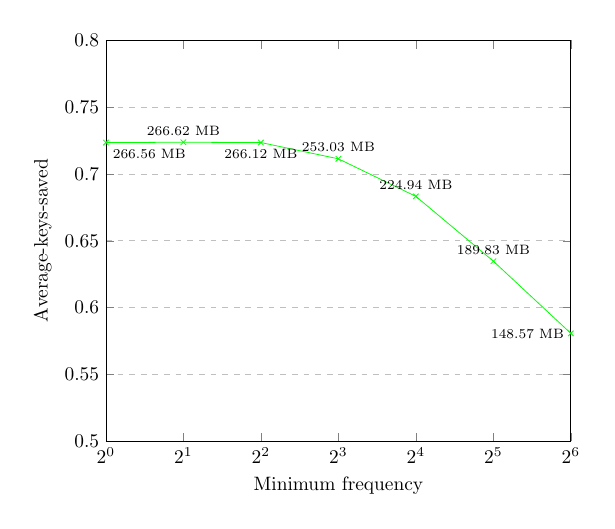
\begin{tikzpicture}[scale=0.7]
	\begin{semilogxaxis}[
		scale only axis,
		xmin=1,xmax=64,
		log basis x=2,
		xtick={1, 2, 4, 8, 16, 32, 64},
		ymin=0.5,ymax=0.8,
		ymajorgrids=true,
		grid style=dashed,
		xlabel=Minimum frequency,
		ylabel=Average-keys-saved]

		\addplot[color=green, mark=x]
		coordinates {(1, 0.72355)(2, 0.72377)(4, 0.72355)(8, 0.71138)(16, 0.68327)(32, 0.63479)(64, 0.58079)};

		\node [below right] at (axis cs:  1, 0.72355) {\scriptsize 266.56 MB};
		\node [above] at (axis cs:  2, 0.72377) {\scriptsize 266.62 MB};
		\node [below] at (axis cs:  4, 0.72355) {\scriptsize 266.12 MB};
		\node [above] at (axis cs:  8, 0.71138) {\scriptsize 253.03 MB};
		\node [above] at (axis cs:  16, 0.68327) {\scriptsize 224.94 MB};
		\node [above] at (axis cs:  32, 0.63479) {\scriptsize 189.83 MB};
		\node [left] at (axis cs:  64, 0.58079) {\scriptsize 148.57 MB};

	\end{semilogxaxis}	
	\end{tikzpicture}
	\caption{3gram + modified Kneser-Ney smoothing}
\end{subfigure}%
\begin{subfigure}{0.5\linewidth}
	\centering
	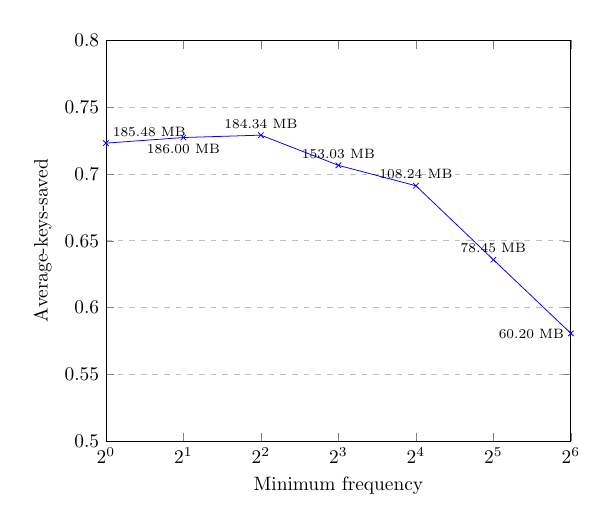
\begin{tikzpicture}[scale=0.7]
	\begin{semilogxaxis}[
		scale only axis,
		xmin=1,xmax=64,
		log basis x=2,
		xtick={1, 2, 4, 8, 16, 32, 64},
		ymin=0.5,ymax=0.8,
		ymajorgrids=true,
		grid style=dashed,
		xlabel=Minimum frequency,
		ylabel=Average-keys-saved]
		
		\addplot[color=blue, mark=x]
		coordinates {(1, 0.72311)(2, 0.72731)(4, 0.72908)(8, 0.70651)(16, 0.69124)(32, 0.63590)(64, 0.58079)};
		
		\node [above right] at (axis cs:  1, 0.72311) {\scriptsize 185.48 MB};
		\node [below] at (axis cs:  2, 0.72731) {\scriptsize 186.00 MB};
		\node [above] at (axis cs:  4, 0.72908) {\scriptsize 184.34 MB};
		\node [above] at (axis cs:  8, 0.70651) {\scriptsize 153.03 MB};
		\node [above] at (axis cs:  16, 0.69124) {\scriptsize 108.24 MB};
		\node [above] at (axis cs:  32, 0.63590) {\scriptsize 78.45 MB};
		\node [left] at (axis cs:  64, 0.58079) {\scriptsize 60.20 MB};
		
	\end{semilogxaxis}
	\end{tikzpicture}
	\caption{Vanilla RNN with 256 hidden neurons}
\end{subfigure}
\caption{The effect of \tit{minimum frequency} and therefore vocabulary size on average-keys-saved and memory usage. Both models were trained using the PTB dataset.}
\end{figure}

\begin{figure}[h]
\captionsetup{justification=centering}
\centering
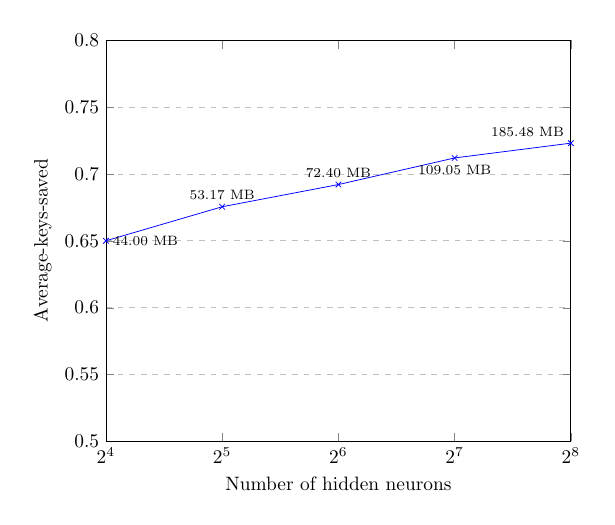
\begin{tikzpicture}[scale=0.7]
\begin{semilogxaxis}[
	scale only axis,
	xmin=16,xmax=256,
	log basis x=2,
	xtick={16, 32, 64, 128, 256},
	ymin=0.5,ymax=0.8,
	ymajorgrids=true,
	grid style=dashed,
	xlabel=Number of hidden neurons,
	ylabel=Average-keys-saved]

	\addplot[color=blue, mark=x]
	coordinates {(16, 0.65007)(32, 0.67552)(64, 0.69212)(128, 0.71204)(256, 0.72310)};
	\node [right] at (axis cs:  16, 0.65007) {\scriptsize 44.00 MB};
	\node [above] at (axis cs:  32, 0.67552) {\scriptsize 53.17 MB};
	\node [above] at (axis cs:  64, 0.69212) {\scriptsize 72.40 MB};
	\node [below] at (axis cs:  128, 0.71204) {\scriptsize 109.05 MB};
	\node [above left] at (axis cs:  256, 0.72310) {\scriptsize 185.48 MB};

\end{semilogxaxis}
\end{tikzpicture}
\caption{The effect of the number of hidden neurons on average-keys-saved and memory usage in a 2-layer vanilla RNN.}
\label{fig:average_keys_saved_vs_number_of_hidden_neurons}
\end{figure}

The vocabulary size was altered by changing a parameter called the \tit{minimum frequency} in my model implementations. This parameter defines the minimum number of times a word must appear in the training set to be considered part of the language model vocabulary. Any words that were not included in the vocabulary were mapped to the unknown-word marker, \ttt{<unk>}. \\

For both the $n$-gram and vanilla RNN models, the minimum frequency can be increased to approximately $2^4$ before the average-keys-saved starts dropping rapidly. In the case of the RNN model, a saving of 77.24 MB is made by increasing the minimum frequency to $2^4$, with a drop of only 0.03187 in average-keys-saved. The savings made on the $n$-gram model are less substantial. \\

From figure~\ref{fig:average_keys_saved_vs_number_of_hidden_neurons}, it can be seen that much greater reductions in memory usage can be achieved for a given loss in average-keys-saved. Dropping from 256 to 32 hidden neurons in each layer gives a memory saving of 132.31 MB, with an average-keys-saved loss of 0.04758. It is intriguing that a 2-layer vanilla RNN with only 32 hidden neurons in each layer can achieve a better average-keys-saved score than the 5-gram model with Katz smoothing from figure~\ref{fig:ptb}. \\

Of course, there are several other techniques that can be used to optimise the memory and CPU overhead of language models for mobile platforms. These include, but are not limited to: using 16-bit floats, rather than 32-bit or 64-bit, to store the model parameters; removing the softmax layer from the RNN, since the outputs do not need to sum to 1 in text prediction; and memory-mapping the model to reduce memory pressure when it is initially being loaded.

\subsection{On Error-Prone Text}

In this section I present my findings for the performance of language models on error-prone text. In the ideal case, when presented with error-prone text, a RNN-based language model should be able to predict the next words that would follow the error-free version of the text, as shown in figure~\ref{fig:error_prone_to_error_free_rnn}.

\begin{figure}[h]
\captionsetup{justification=centering}
\centering
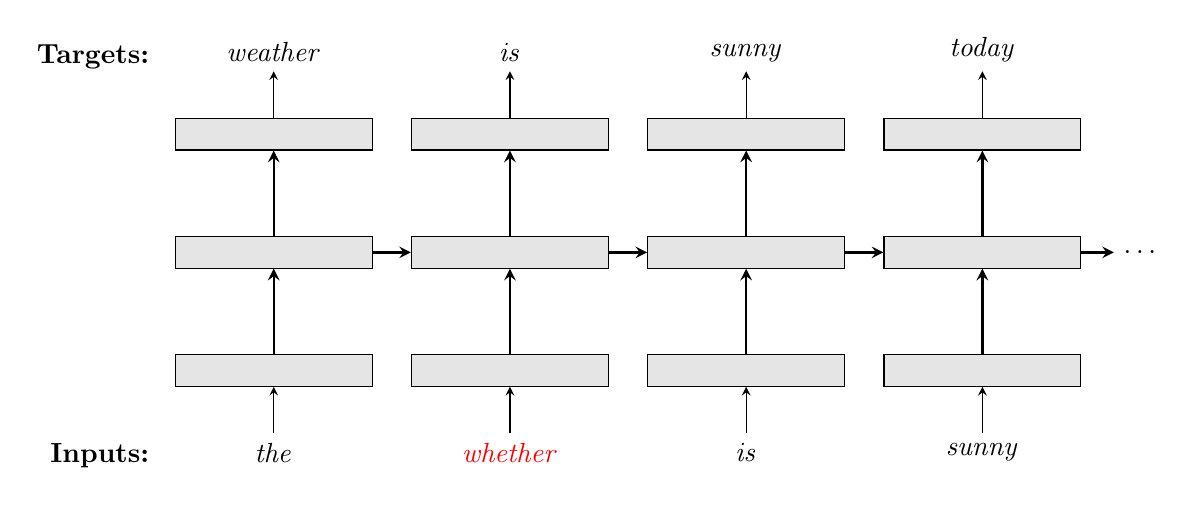
\begin{tikzpicture}[>=stealth]
	\node[draw, rectangle, minimum width=25mm, minimum height=4mm, fill=black!10, ] (input1) at (0, 0) {};
	\node[draw, rectangle, minimum width=25mm, minimum height=4mm, fill=black!10] (hidden1) at (0, 1.5) {};
	\node[draw, rectangle, minimum width=25mm, minimum height=4mm, fill=black!10] (output1) at (0, 3) {};
	\draw [<-] (input1) -- ++(0, -0.8) node [below] {\tit{the}};
	\draw [->, line width=0.3mm] (input1) -- (hidden1);
	\draw [->, line width=0.3mm] (hidden1) -- (output1);
	\draw [->] (output1) -- ++(0, 0.8) node [above] {\tit{weather}};
	
	\node[below left=6mm and 2mm of input1] (inputs) {\tbf{Inputs:}};
	\node[above left=5mm and 2mm of output1] (targets) {\tbf{Targets:}};

	\node[draw, rectangle, minimum width=25mm, minimum height=4mm, fill=black!10, ] (input2) at (3, 0) {};
	\node[draw, rectangle, minimum width=25mm, minimum height=4mm, fill=black!10] (hidden2) at (3, 1.5) {};
	\node[draw, rectangle, minimum width=25mm, minimum height=4mm, fill=black!10] (output2) at (3, 3) {};
	\draw [<-] (input2) -- ++(0, -0.8) node [below] {\textcolor{red}{\tit{whether}}};
	\draw [->, line width=0.3mm] (input2) -- (hidden2);
	\draw [->, line width=0.3mm] (hidden2) -- (output2);
	\draw [->] (output2) -- ++(0, 0.8) node [above] {\tit{is}};

	\node[draw, rectangle, minimum width=25mm, minimum height=4mm, fill=black!10, ] (input3) at (6, 0) {};
	\node[draw, rectangle, minimum width=25mm, minimum height=4mm, fill=black!10] (hidden3) at (6, 1.5) {};
	\node[draw, rectangle, minimum width=25mm, minimum height=4mm, fill=black!10] (output3) at (6, 3) {};
	\draw [<-] (input3) -- ++(0, -0.8) node [below] {\tit{is}};
	\draw [->, line width=0.3mm] (input3) -- (hidden3);
	\draw [->, line width=0.3mm] (hidden3) -- (output3);
	\draw [->] (output3) -- ++(0, 0.8) node [above] {\tit{sunny}};
	
	\node[draw, rectangle, minimum width=25mm, minimum height=4mm, fill=black!10, ] (input4) at (9, 0) {};
	\node[draw, rectangle, minimum width=25mm, minimum height=4mm, fill=black!10] (hidden4) at (9, 1.5) {};
	\node[draw, rectangle, minimum width=25mm, minimum height=4mm, fill=black!10] (output4) at (9, 3) {};
	\draw [<-] (input4) -- ++(0, -0.8) node [below] {\tit{sunny}};
	\draw [->, line width=0.3mm] (input4) -- (hidden4);
	\draw [->, line width=0.3mm] (hidden4) -- (output4);
	\draw [->] (output4) -- ++(0, 0.8) node [above] {\tit{today}};

	\node (cont) at (11, 1.5) {$\hdots$};

	\draw [->, line width=0.3mm] (hidden1.east) -- (hidden2.west);
	\draw [->, line width=0.3mm] (hidden2.east) -- (hidden3.west);
	\draw [->, line width=0.3mm] (hidden3.east) -- (hidden4.west);
	\draw [->, line width=0.3mm] (hidden4.east) -- (cont.west);
\end{tikzpicture}
\caption{The ideal language model that can make predictions regardless of errors in the input text.}
\label{fig:error_prone_to_error_free_rnn}
\end{figure}

Normally, language models are evaluated by feeding them a sequence of input words (\tit{the inputs}) and seeing how well they predict that same sequence of input words shifted forward in time by one word (\tit{the targets}). When evaluating my error-correcting language models, I did exactly the same thing, except that the inputs were allowed to contain error in them and the targets were not. \\

In order to obtain sequences of words with and without errors in them I used the CLC dataset. I split this dataset up into six files:
\begin{center}
\begin{tabular}{c c}
	\ttt{train.correct.txt} & \ttt{train.incorrect.txt} \\
	\ttt{valid.correct.txt} & \ttt{valid.incorrect.txt} \\
	\ttt{test.correct.txt} & \ttt{test.incorrect.txt}
\end{tabular}
\end{center}
The training, validation and test sets all consisted of one file containing uncorrected text and another file containing the corresponding corrected text. I trained an 2-layer LSTM-based language model with 256 hidden neurons on \ttt{train.correct.txt}, and used \ttt{valid.correct.txt} to guide the learning rate decay. In order to focus the evaluation on the error-correcting ability of my language models, I removed any pairs of lines from the test set files that were identical. I also removed any pairs of lines that contained corrections that involve the insertion or deletion of words, because my model was not designed to handle these types of errors, as explained in section~\ref{error_correcting_lm}. \\

Before exploring ways to improve predictions on error-prone text, I first established an approximate lower and upper bound on the performance. The ideal error-correcting language model would predict words as if the input were not error-prone, therefore, to obtain the upper bound in performance, I evaluated the LSTM-based language model using \ttt{test.correct.txt} for the input words and \ttt{test.correct.txt} for the target words. In order to establish a lower bound, I evaluated the performance of the same model using \ttt{test.incorrect.txt} for the input words and \ttt{test.correct.txt} for the target words. This model did not contain any error-correcting capabilities. \\

As explained in section~\ref{error_correcting_lm}, my error-correcting language model attempted to replace words in the context that were not contained in a dictionary of English words, by going through the language model vocabulary in order of decreasing probability and picking the first candidate word within an edit distance $\delta$ of the original word. \\

\begin{figure}[h]
\captionsetup{justification=centering}
\begin{adjustbox}{center}
\begin{tabular}{| L{3.5cm} | L{8cm} | C{2.2cm} | C{2cm} |}
	\hline
	\tbf{Language model} & \tbf{Description} & \tbf{Perplexity} & \tbf{Average-keys-saved} \\ \hline
	\tit{Upper bound} & The best performance achievable assuming perfect error-correction. & 77.83 & 0.65483 \\ \hline
	\tit{Error-correcting LSTM} & $\delta$ = 1 & 87.99 & 0.64453 \\ \hline
	\tit{Error-correcting LSTM} & $\delta$ = 2 & 88.47 & 0.64376 \\ \hline
	\tit{Error-correcting LSTM} & $\delta$ = 3 & 88.57 & 0.64273 \\ \hline
	\tit{Lower bound} & The performance that would be achieved with no error-correction. & 89.70 & 0.63912 \\ \hline
\end{tabular}
\end{adjustbox}
\caption{The performance of my error-correcting language model with respect to the upper and lower bound, using the CLC dataset.}
\label{fig:error_correcting_results}
\end{figure}

It can be seen from figure~\ref{fig:error_correcting_results} that this approach improves the performance of language model predictions on error-prone text, with the best result arising from an edit distance of 1. There is, however, still a gap between this performance and the theoretical upper bound. The reasoning why this gap exists can be understood by looking at the corrections that the language model did make, and the corrections that it failed to make. \\

\todo{Show sample corrections, explain why $D=V$ isn't good and explain what errors aren't covered.}

\chapter{Conclusions}

The project was a success: I implemented a variety of $n$-gram and RNN-based language models, and benchmarked them in terms of both their prediction performance and their applicability to running on a mobile platform, as set out in my project proposal. Additionally, I built a mobile keyboard for iOS that uses my language models as a library, and proposed a novel extension to an existing language model that improves its performance on error-prone text. \\

Conclusions:
\begin{itemize}
\item
	Neural models offer best performance, but take longest to train.
\item
	Significant prediction improvements can be achieved by interpolating language models.
\item
	Memory reduction is most effectively achieved by reducing the number of hidden neurons.
\item
	Best option for mobile device is perhaps to combine one or more memory-reduced language models.
\end{itemize}

In my project, I explicitly demonstrated that language model performance is deterred by error-prone text. Whilst I made some modifications to an existing model that saw an increase in performance on such text, there is still room for improvement. If I were given more time to work on the project, I would investigate ways to cater for non-spelling corrections, and changes that involve the insertion or deletion of words.

Future work/possible extensions:
\begin{itemize}
\item
	More intelligent ways of pruning $n$-gram models.
\item
	Using Neural Machine Translation to correct the context, making use of attention.	
\end{itemize}

%%%%%%%%%%%%%%%%%%%%%%%%%%%%%%%%%%%%%%%%%%%%%%%%%%%%%%%%%%%%%%%%%%%%%
% the bibliography
\addcontentsline{toc}{chapter}{Bibliography}
\bibliographystyle{ieeetr}
\bibliography{bibliography}

%%%%%%%%%%%%%%%%%%%%%%%%%%%%%%%%%%%%%%%%%%%%%%%%%%%%%%%%%%%%%%%%%%%%%
% the appendices
\appendix

\chapter{Backpropagation Recurrence Relation} \label{appendix:bp_recurrence}

\begin{align*}
	\delta_i^l &= \sum_j \delta_j^{l+1} \frac{\partial z_j^{l+1}}{\partial z_i^l} \\
	&= \sum_j \delta_j^{l+1} \frac{\partial z_j^{l+1}}{\partial y_i^l} \frac{\partial y_i^l}{\partial z_i^l} \\
	&= \sum_j \delta_j^{l+1} w_{i,j}^l \phi'(z_i^l) \\
	&= \phi'(z_i^l) \sum_j \delta_j^{l+1} w_{i,j}^l \\
\end{align*}

\chapter{Project Proposal}

\end{document}
